\documentclass{article}
% \usepackage[headsepline]{scrlayer-scrpage}

% \ihead{Levin}
% \ohead{\thepage}
% \pagestyle{scrheadings}
\usepackage{bbm}
\usepackage{amsmath,amsfonts,amsthm,amssymb,amsopn,bm}
\usepackage[margin=.9in]{geometry}
\usepackage{graphicx}
\usepackage{url}
\usepackage[usenames,dvipsnames]{color}
\usepackage{fancyhdr}
\usepackage{multirow}
\usepackage{pythonhighlight}
\usepackage{pgfplots}
\usepackage{pgfplots}
\pgfplotsset{compat=1.11}
\usepackage{minted}
% Default fixed font does not support bold face
\DeclareFixedFont{\ttb}{T1}{txtt}{bx}{n}{12} % for bold
\DeclareFixedFont{\ttm}{T1}{txtt}{m}{n}{12}  % for normal

% Custom colors
\usepackage{color}
\definecolor{deepblue}{rgb}{0,0,0.5}
\definecolor{deepred}{rgb}{0.6,0,0}
\definecolor{deepgreen}{rgb}{0,0.5,0}

\usepackage{listings}

% Python style for highlighting
\newcommand\pythonstyle{\lstset{
language=Python,
basicstyle=\ttm,
otherkeywords={self},             % Add keywords here
keywordstyle=\ttb\color{deepblue},
emph={MyClass,__init__},          % Custom highlighting
emphstyle=\ttb\color{deepred},    % Custom highlighting style
stringstyle=\color{deepgreen},
frame=tb,                         % Any extra options here
showstringspaces=false            % 
}}


% Python environment
\lstnewenvironment{python}[1][]
{
\pythonstyle
\lstset{#1}
}
{}

% Python for external files
\newcommand\pythonexternal[2][]{{
\pythonstyle
\lstinputlisting[#1]{#2}}}

% Python for inline
\newcommand\pythoninline[1]{{\pythonstyle\lstinline!#1!}}

% Some additional tweaking for this package can be made in the preamble. To change the size of each plot and also guarantee backwards compatibility (recommended) add the next line:

\pgfplotsset{width=10cm,compat=1.9}

% This changes the size of each pgfplot figure to 10 centimeters, which is huge; you may use different units (pt, mm, in). The compat parameter is for the code to work on the package version 1.9 or later.

% Since LaTeX was not initially conceived with plotting capabilities in mind, when there are several pgfplot figures in your document or they are very complex, it takes a considerable amount of time to render them. To improve the compiling time you can configure the package to export the figures to separate PDF files and then import them into the document, add the code shown below to the preamble:

\usepgfplotslibrary{external}

\tikzexternalize 

\newcommand{\field}[1]{\mathbb{#1}}
\newcommand{\1}{\mathbf{1}}
\newcommand{\I}{\mathbbm{1}}
\newcommand{\E}{\mathbb{E}} 
\newcommand{\V}{\mathbb{V}} 
\renewcommand{\P}{\mathbb{P}}
 \newcommand{\ind}{\perp\!\!\!\perp}
 \DeclareMathOperator{\rank}{rank}
\newcommand{\R}{\field{R}} % real domain
% \newcommand{\C}{\field{C}} % complex domain
\newcommand{\F}{\field{F}} % functional domain

\newcommand{\T}{^{\textrm T}} % transpose

\def\diag{\text{diag}}

%% operator in linear algebra, functional analysis
\newcommand{\inner}[2]{#1\cdot #2}
\newcommand{\norm}[1]{\left\|#1\right\|}
\newcommand{\twonorm}[1]{\|#1\|_2^2}
% operator in functios, maps such as M: domain1 --> domain 2
\newcommand{\Map}[1]{\mathcal{#1}}
\renewcommand{\theenumi}{\alph{enumi}} 

\newcommand{\Perp}{\perp \! \! \! \perp}

\newcommand\independent{\protect\mathpalette{\protect\independenT}{\perp}}
\def\independenT#1#2{\mathrel{\rlap{$#1#2$}\mkern2mu{#1#2}}}
\newcommand{\vct}[1]{\boldsymbol{#1}} % vector
\newcommand{\mat}[1]{\boldsymbol{#1}} % matrix
\newcommand{\cst}[1]{\mathsf{#1}} % constant
\newcommand{\ProbOpr}[1]{\mathbb{#1}}
\newcommand{\points}[1]{\small\textcolor{magenta}{\emph{[#1 points]}} \normalsize}
\date{{}}

\setlength\parindent{0px}

\begin{document}
\title{Homework \#2}
\author{\normalsize{Spring 2020, CSE 546: Machine Learning}\\
\normalsize{\bf Roman Levin} \\
\normalsize{\bf 1721898} \\
}
\maketitle
Collaborators: compared answers with Tyler Chen, Diya Sashidhar, Katherine Owens

\subsection*{Conceptual Questions}
\noindent\rule{\textwidth}{1pt}

A.0 {\bf Solution:}\\
\begin{enumerate}
    \item {\bf No,} because there could be several perfectly correlated features, each with large positive weight (e.g. 'number of bathrooms' and 'number of showers'). If they are perfectly correlated, then either one could be removed without compromising the quality of the predictions.
    \item Because of {\bf the shape of L1 and L2 norm balls (level sets)}. The L1 ball is more "spiky" (with sparse vertices) and therefore level sets of the original objective are more likely to intersect it at its sparse vertices (unlike in the case of L2) resulting in a sparse solution to the regularized problem. Also, L0 penalty explicitly penalizes the number of non-zero elements and, between $p = 2$ and $p = 1$, the latter is closer to $p = 0$, and thus L1 norm is a better proxy for L0 than L2 is.
    \item Upside: promotes {\bf sparsity} even better than L1. Downside: {\bf non-convex}.
    \item {\bf True}
    \item Because {\bf in expectation it goes in the right direction.}
    \item Advantage: one iteration of SGD {\bf is much less expensive computationally} compared to GD. Disadvantage: SGD requires {\bf more iterations} to reach the same error.
\end{enumerate}

\noindent\rule{\textwidth}{1pt}
\subsection*{Convexity and Norms}
\noindent\rule{\textwidth}{1pt}
A.1 {\bf Solution:}\\
\begin{enumerate}
    \item First, let's prove the following (obvious) fact: $\forall a,b \in \R: |a + b| \le |a| + |b|$:
    $$|a + b|^2 = a^2 + b^2 + 2ab \le a^2 + b^2 + 2|a||b| = (|a| + |b|)^2 \Rightarrow |a + b| \le |a| + |b| \text{  since  } |a + b|\ge 0, |a| + |b|\ge 0. \Box$$
    Now, let's check the definition of the norm for L1 norm $f(x) = \sum_{i=1}^n |x_i|$:
    \begin{itemize}
        \item (Non-negativity): $f(x) \ge 0$ since $\forall i: |x_i| \ge 0$. Now, $|x_i| = 0$ iff $x_i = 0$, so $f(x) = 0$ iff $x = 0$. $\Box$
        \item (Absolute scalability): $\forall a\in \R, x\in \R^n: f(ax) = \sum_{i=1}^n |ax_i| = \sum_{i=1}^n |a||x_i| = |a|f(x). \Box$
        \item (Triangle inequality): $\forall x,y \in \R^n: f(x) + f(y) = \sum_{i=1}^n |x_i| + \sum_{i=1}^n |y_i| = \sum_{i=1}^n |x_i| + |y_i| \ge \sum_{i=1}^n |x_i + y_i| = f(x+y)$, where the second to last inequality follows from the triangle inequality for absolute values on $\R$ above. $\Box$
    \end{itemize}
    \item Consider $x = [0, 1]^T, y = [1, 0]^T$. Then $g(x) + g(y) = 1^2 + 1^2 = 2, g(x+y) = (1 + 1)^2 = 4$, so for these $x,y$: $g(x+y) > g(x) + g(y)$ and the triangle inequality does not hold which means $g$ is not a norm. $\Box$
    
\end{enumerate}

\noindent\rule{\textwidth}{1pt}


\noindent\rule{\textwidth}{1pt}
B.1 {\bf Solution:}\\
\begin{itemize}
    \item Note that $\max_i (|x_i|^2) = (\max_i |x_i|)^2$ since $|x_i| \ge 0$. Now 
    $$
    \|x\|_2^2 = \sum_i|x_i|^2 \ge \max_i (|x_i|^2) = (\max_i |x_i|)^2 = \|x\|^2_{\infty} \Leftrightarrow \|x\|_2 \ge \|x\|_{\infty} \text{  since  } \|x\|_2\ge0, \|x\|_{\infty}\ge0.
    $$
    \item $\|x\|_1^2 = (\sum_i |x_i|)^2 = \sum_i |x_i|^2 + \underbrace{\sum_{i\not=j} |x_i||x_j|}_{\ge 0} \ge \sum_i |x_i|^2 = \|x\|_2^2 \Leftrightarrow \|x\|_1 \ge \|x\|_2$ since $\|x\|_2\ge0, \|x\|_1\ge0$
    \item That is, $\boxed{\|x\|_1 \ge \|x\|_2 \ge \|x\|_{\infty}. \Box}$
\end{itemize}
\noindent\rule{\textwidth}{1pt}

\noindent\rule{\textwidth}{1pt}
A.2 {\bf Solution:}\\
\begin{itemize}
    \item {\bf I is not convex}: line segment between points $b$ and $c$ is not in the set, while the points are. 
    \item {\bf II is convex.} 
    \item {\bf III is not convex}: line segment between points $d$ and $a$ is not in the set, while the points are.
\end{itemize}
\noindent\rule{\textwidth}{1pt}

\noindent\rule{\textwidth}{1pt}
\\
A.3 {\bf Solution:}\\
\begin{enumerate}
    \item {\bf I is convex} on $[a,c[$.
    \item {\bf II is not convex} on $[a,c]$: for $\lambda = 1/2$: $f(\lambda b + (1-\lambda)c) > \lambda f(b) + (1-\lambda)f(c)$. 
    \item {\bf III is convex} on $[a,d]$: for $\lambda = 1/2$: $f(\lambda a + (1-\lambda)c) > \lambda f(a) + (1-\lambda)f(c)$
    \item {\bf III is convex} on $[c,d]$.
\end{enumerate}   
\noindent\rule{\textwidth}{1pt}

\noindent\rule{\textwidth}{1pt}
\\
B.2 {\bf Solution:}\\
\begin{enumerate}
    \item We will show convexity by definition. Take any $\lambda \in [0,1]$. Note that $(1-\lambda) \in [0,1]$. Then, taking any $x, y \in \R^n$, by triangle inequality and absolute scalability:
    $$
    \|\lambda x + (1-\lambda)y\| \le \|\lambda x\| + \|(1-\lambda)y\| \le \lambda\|x\| + (1-\lambda)\|y\| \Box.
    $$
    \item $B := \{x \in \R^n: \|x\| \le 1\}$. Take any $\lambda \in [0,1]$ and any $x,y \in B$. Then (using derivations in a.):
    $$
    \|\lambda x + (1-\lambda)y\| \le \lambda\underbrace{\|x\|}_{\le 1 \text{ for } x \in B} + (1-\lambda)\underbrace{\|y\|}_{\le 1 \text{ for } y \in B} \le \lambda + 1 - \lambda = 1 \Rightarrow \lambda x + (1-\lambda)y \in B 
    $$
    So $B$ is indeed a convex set. $\Box$
    \item The plot of $L:=\{(x,y): g(x,y) \le 4\}$, where $g(x,y) = (|x|^{1/2} + |y|^{1/2})^2$ is on Figure 1. This set is not convex because for $\lambda = 0.5$ and points $x = [0,-4]^T, y =[4,0]^T, x,y \in L$:
    $$\lambda x + (1-\lambda)y \not\in L \Box$$
    
   
    \begin{figure}[h!]
            \centering
            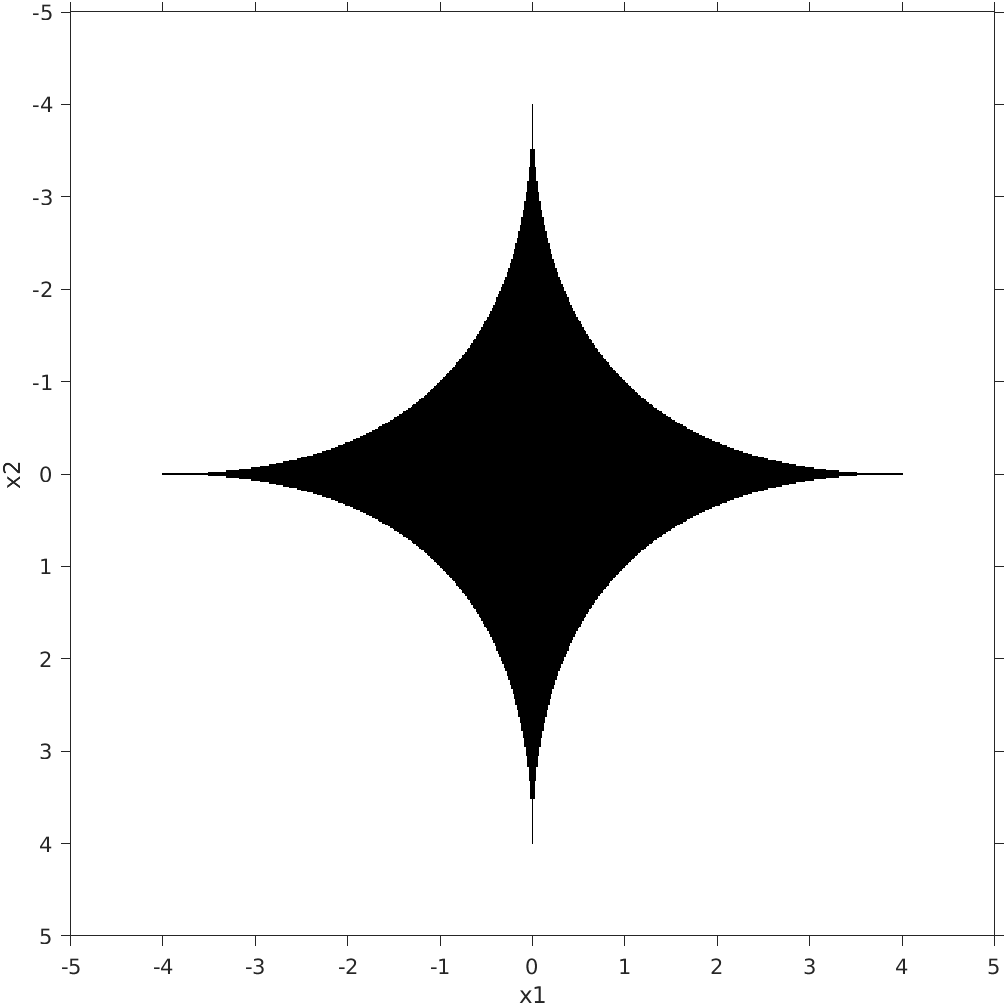
\includegraphics[width=0.4\textwidth]{hw2/b2.png}
            \caption{Plot of $\{(x,y): g(x,y) \le 4\}$, where $g(x,y) = (|x|^{1/2} + |y|^{1/2})^2$}
            \label{figure:B2}
    \end{figure}
\end{enumerate}   
\noindent\rule{\textwidth}{1pt}

\noindent\rule{\textwidth}{1pt}
\\
B.3 {\bf Solution:}\\
\begin{enumerate}
    \item 
    \begin{itemize}
        \item  Let's first show that the sum of convex functions is convex. Let $f,g$ be convex, consider $f(x) + g(x)$. Take any $\lambda \in [0,1]$, take any $x, y$. Then, by convexity of $f$ and $g$:
        $$
        f(\lambda x + (1-\lambda)y) + g(\lambda x + (1-\lambda)y) \le \lambda f(x) + (1-\lambda)f(y) + \lambda g(x) + (1-\lambda)g(y) = \lambda (f(x) + g(x)) + (1-\lambda)(f(y) + g(y)). \Box
        $$
        That is, $f(x) + g(x)$ is convex if $f(x)$ and $g(x)$ are convex. Now, a sum $\sum_{i=1}^n f_i(x)$ of $n$ convex functions $f_i(x)$ is also convex because by the above we can first show that $f_1(x) + f_2(x)$ is convex, that implies the convexity of $f_1(x) + f_2(x) + f_3(x)$, etc. At every step $j$, we know that $\sum_{i=1}^{j}f_i(x)$ is convex and $f_{j+1}(x)$ is also convex, so $\sum_{i=1}^{j+1}f_i(x)$ is convex. That is, by induction, it follows that $\sum_{i=1}^n f_i(x)$ is convex. $\Box$
        \item Now, multiplication by $\lambda > 0$ obviously preserves convexity and thus $\lambda\|w\|$ is convex because $\|w\|$ is convex. To see that, take any $\alpha \in [0,1]$ and any $x,y$:
        $$
        \lambda\|\alpha x + (1-\alpha)y\| \le \lambda(\alpha\|x\| + (1-\alpha)\|y\|) = \alpha\lambda\|x\| + (1-\alpha)\lambda\|y\|
        $$
        \item Finally, since $l_i(w) \text{ are convex } \Rightarrow \sum_{i=1}^n l_i(w)$ is convex. As shown above, $\lambda \|w\|$ is convex too. So 
        $\sum_{i=1}^n l_i(w) + \lambda \|w\|$ is convex as a sum of two convex functions. $\Box$
    \end{itemize}
    \item Because convexity implies that every local minimum is a global minimum. $\Box$
\end{enumerate}   
\noindent\rule{\textwidth}{1pt}


\subsection*{Lasso}

\noindent\rule{\textwidth}{1pt}
A.4 {\bf Solution:}\\
\begin{enumerate}
    \item See Plot 1 in Figure 2 (left). Note that for this problem I treated numbers less than 1e-14 in absolute value as zeros.
    \item See Plot 2 in Figure 2 (right). 
        \begin{figure}[h!]
            \centering
            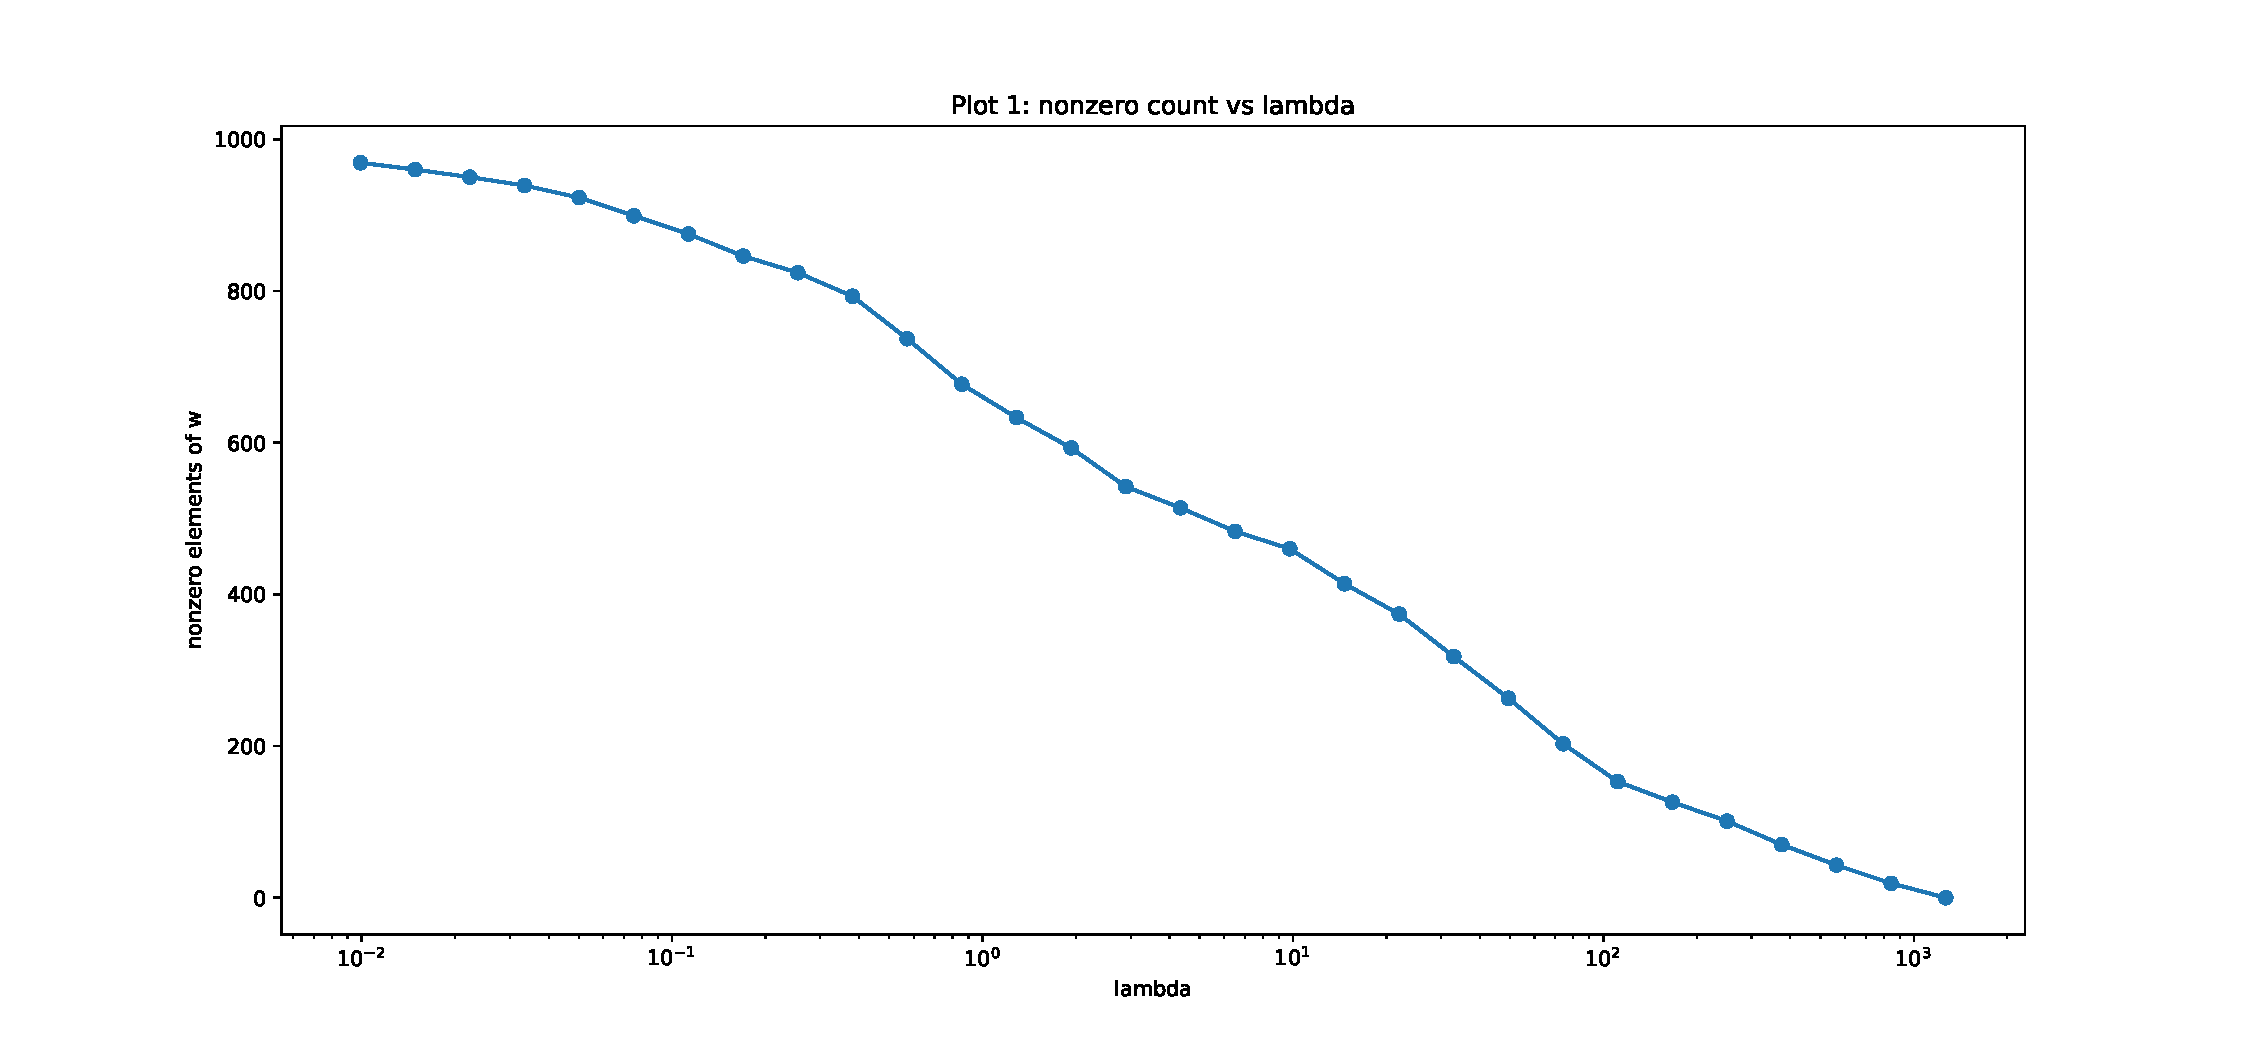
\includegraphics[width=0.45\textwidth]{hw2/code/figures/A4a.pdf}
            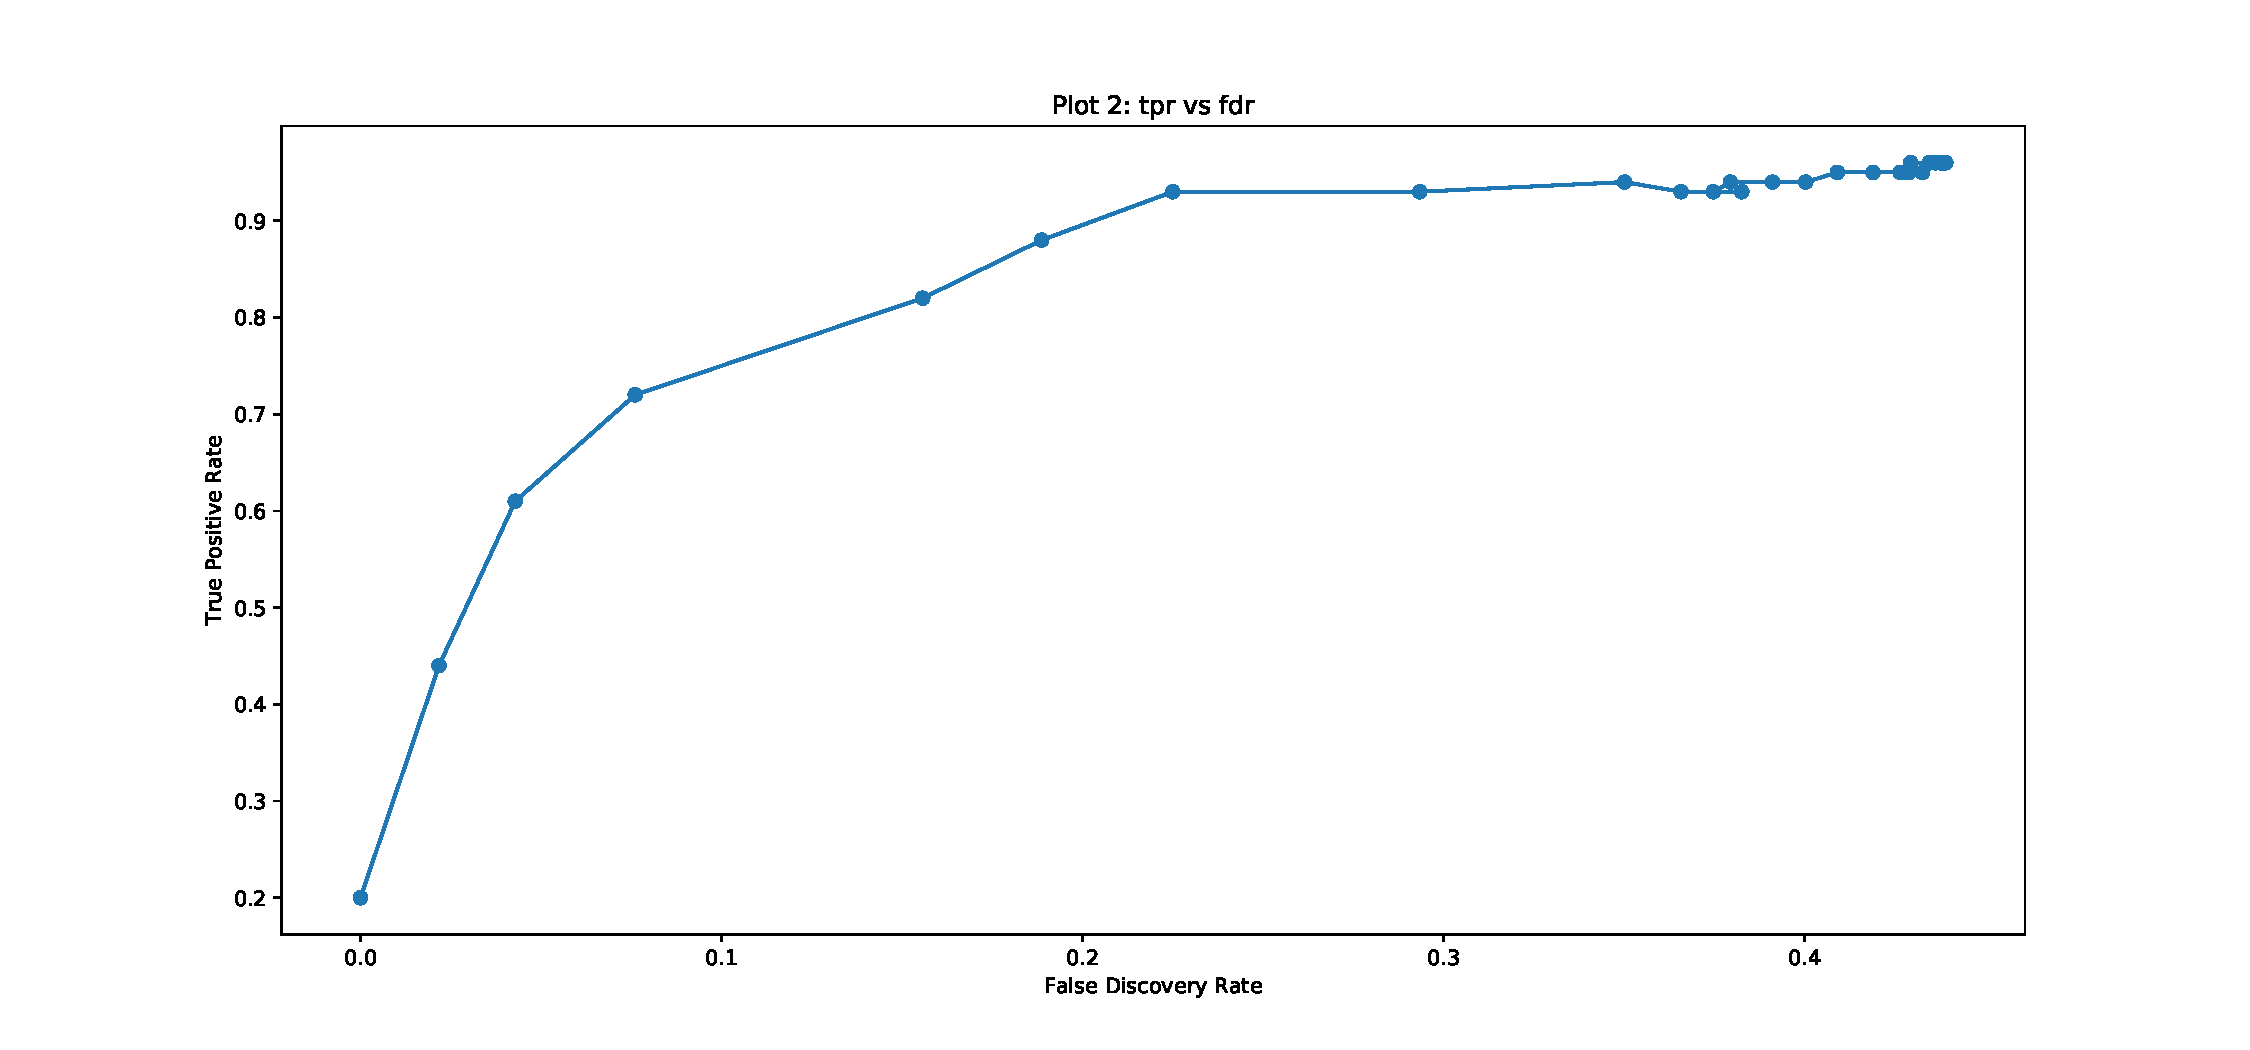
\includegraphics[width=0.45\textwidth]{hw2/code/figures/A4b.pdf}
            \caption{Problem A4. Left: A4.a, Right: A4.b}
            \label{figure:a4}
        \end{figure}
    \item From the plots we see, as expected, that greater $\lambda$ forces more weights to zero. That is, increasing $\lambda$ results in a more sparse solution. However, in Plot 2, we see that too large $\lambda$ results in zero solution which gives poor performance. If we use $\lambda$ which is too small, we end up in another extreme, where we have a high false discovery rate. One should choose $\lambda$ which is close to the upper left corner on Plot 2. (Probably, making this plot on a validation set would be a good idea too for choosing $\lambda$).
\end{enumerate}
\inputminted{python}{code/A4.py}
\caption{Code for A4}
\noindent\rule{\textwidth}{1pt}



\noindent\rule{\textwidth}{1pt}
A.5 {\bf Solution:}\\
\begin{enumerate}
    \item See Figure 3 (top left). 
    \item See Figure 3 (top right). 
    \item See Figure 3 (bottom).
        \begin{figure}[h!]
            \centering
            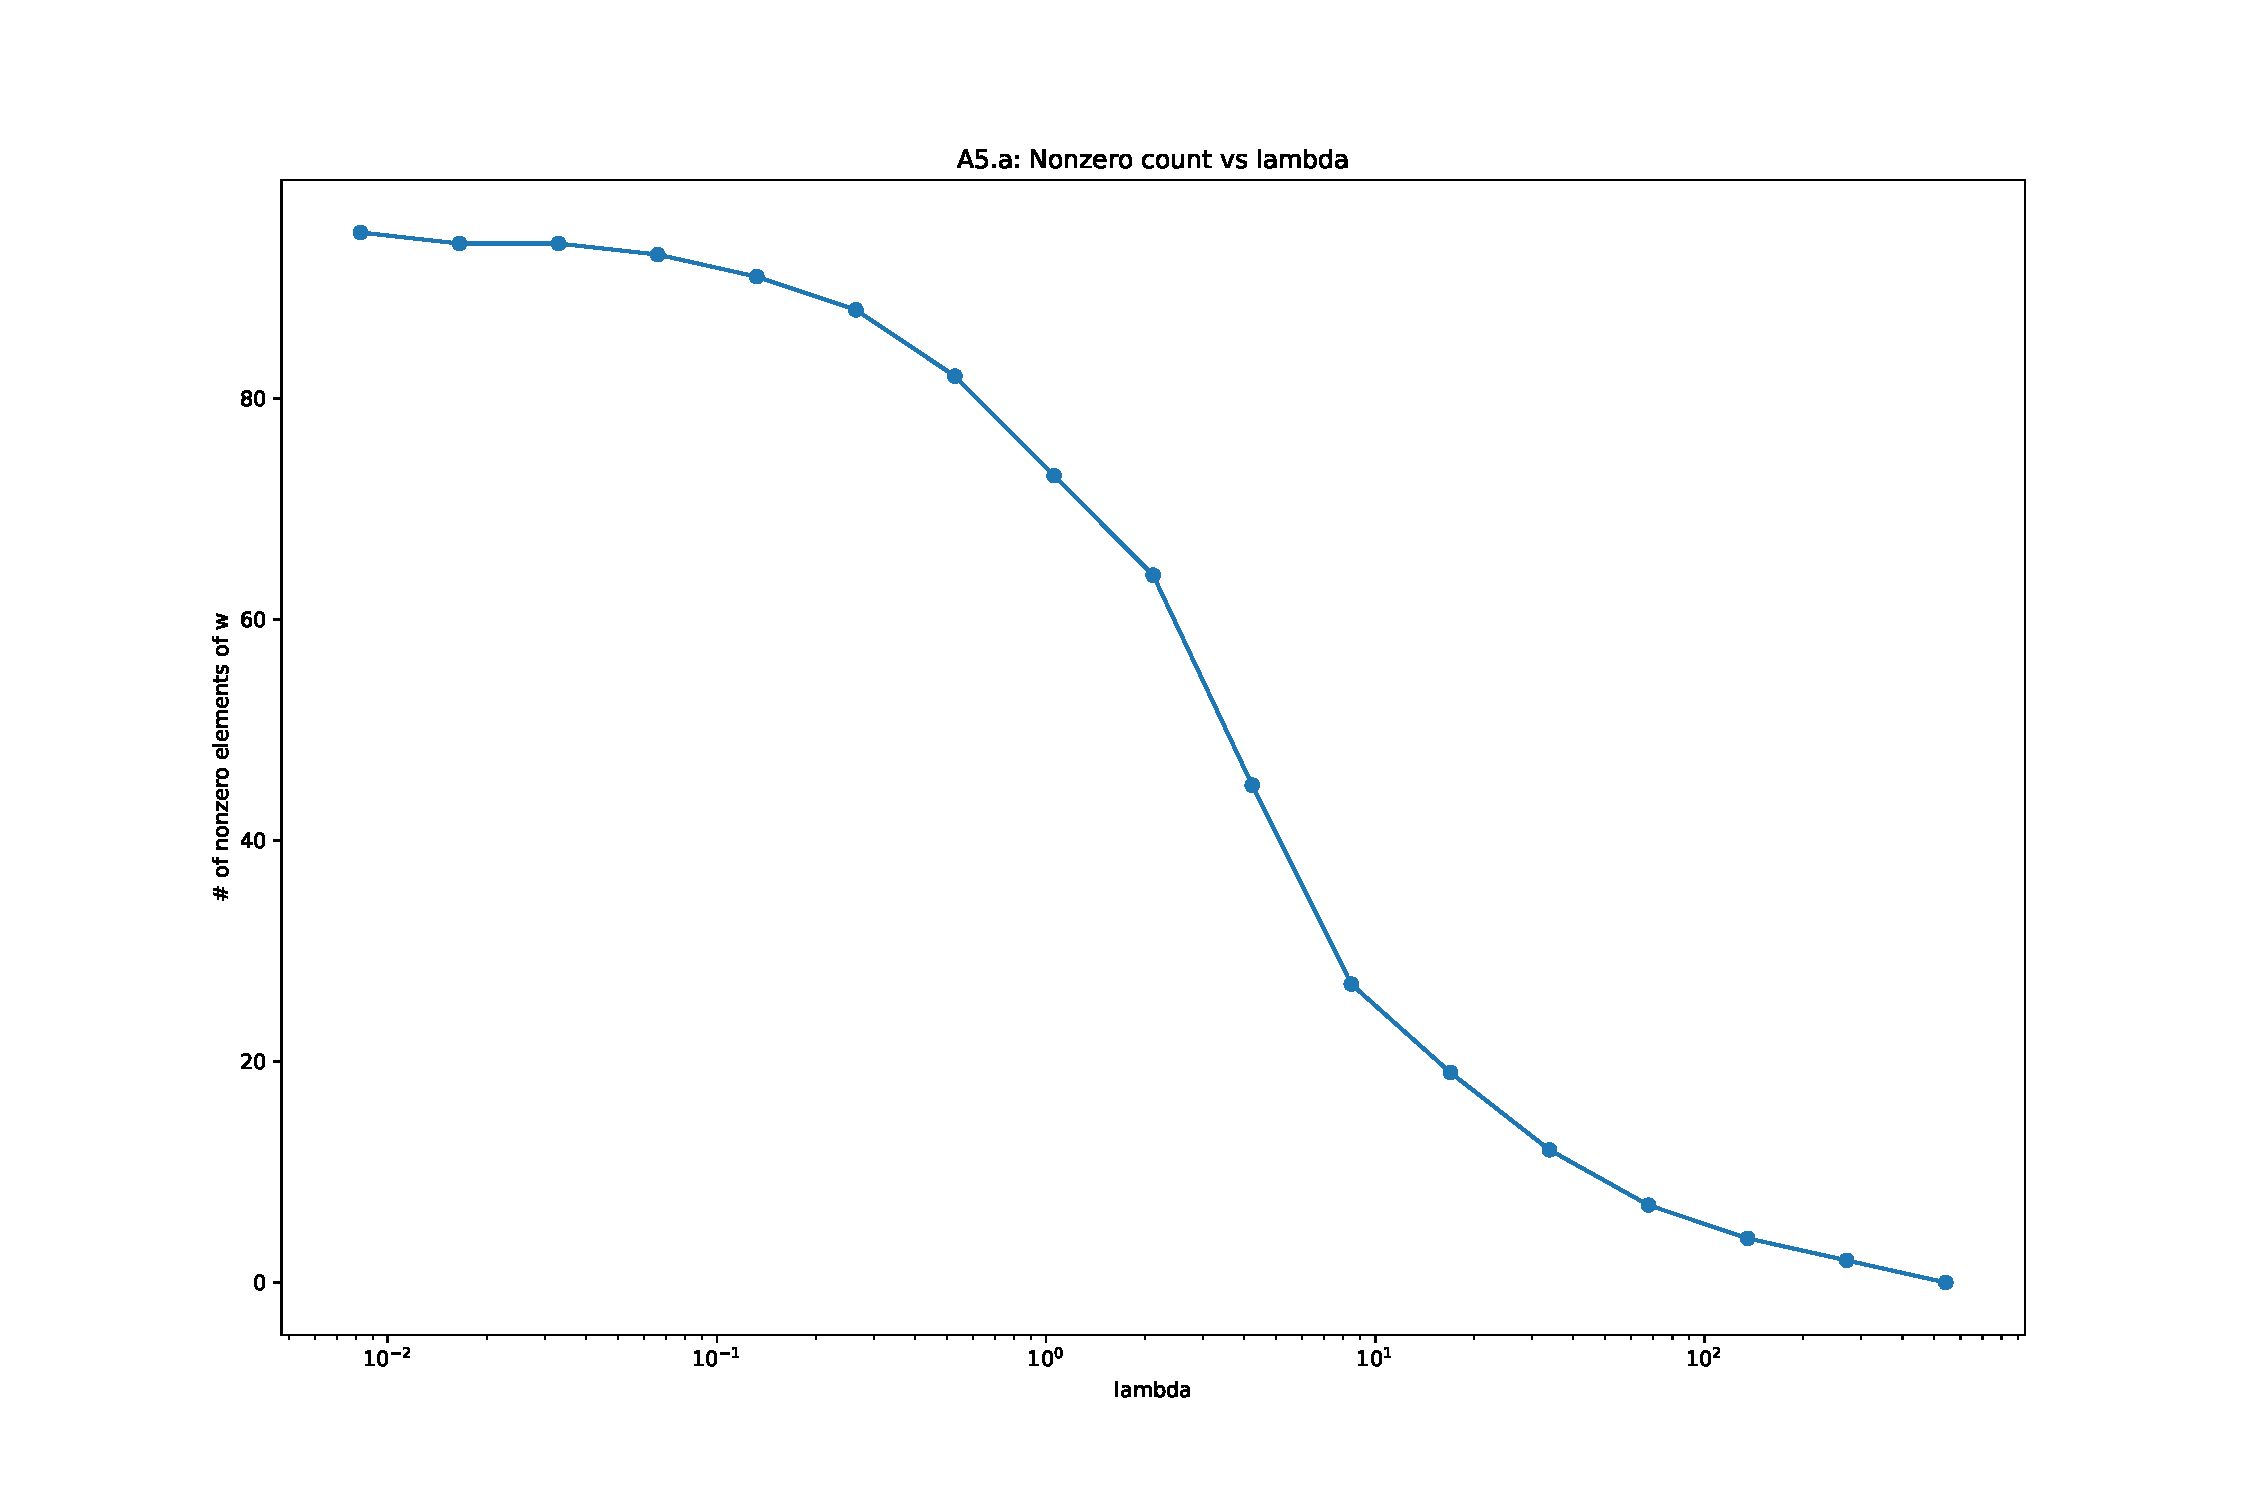
\includegraphics[width=0.49\textwidth]{hw2/code/figures/A5a.pdf}
            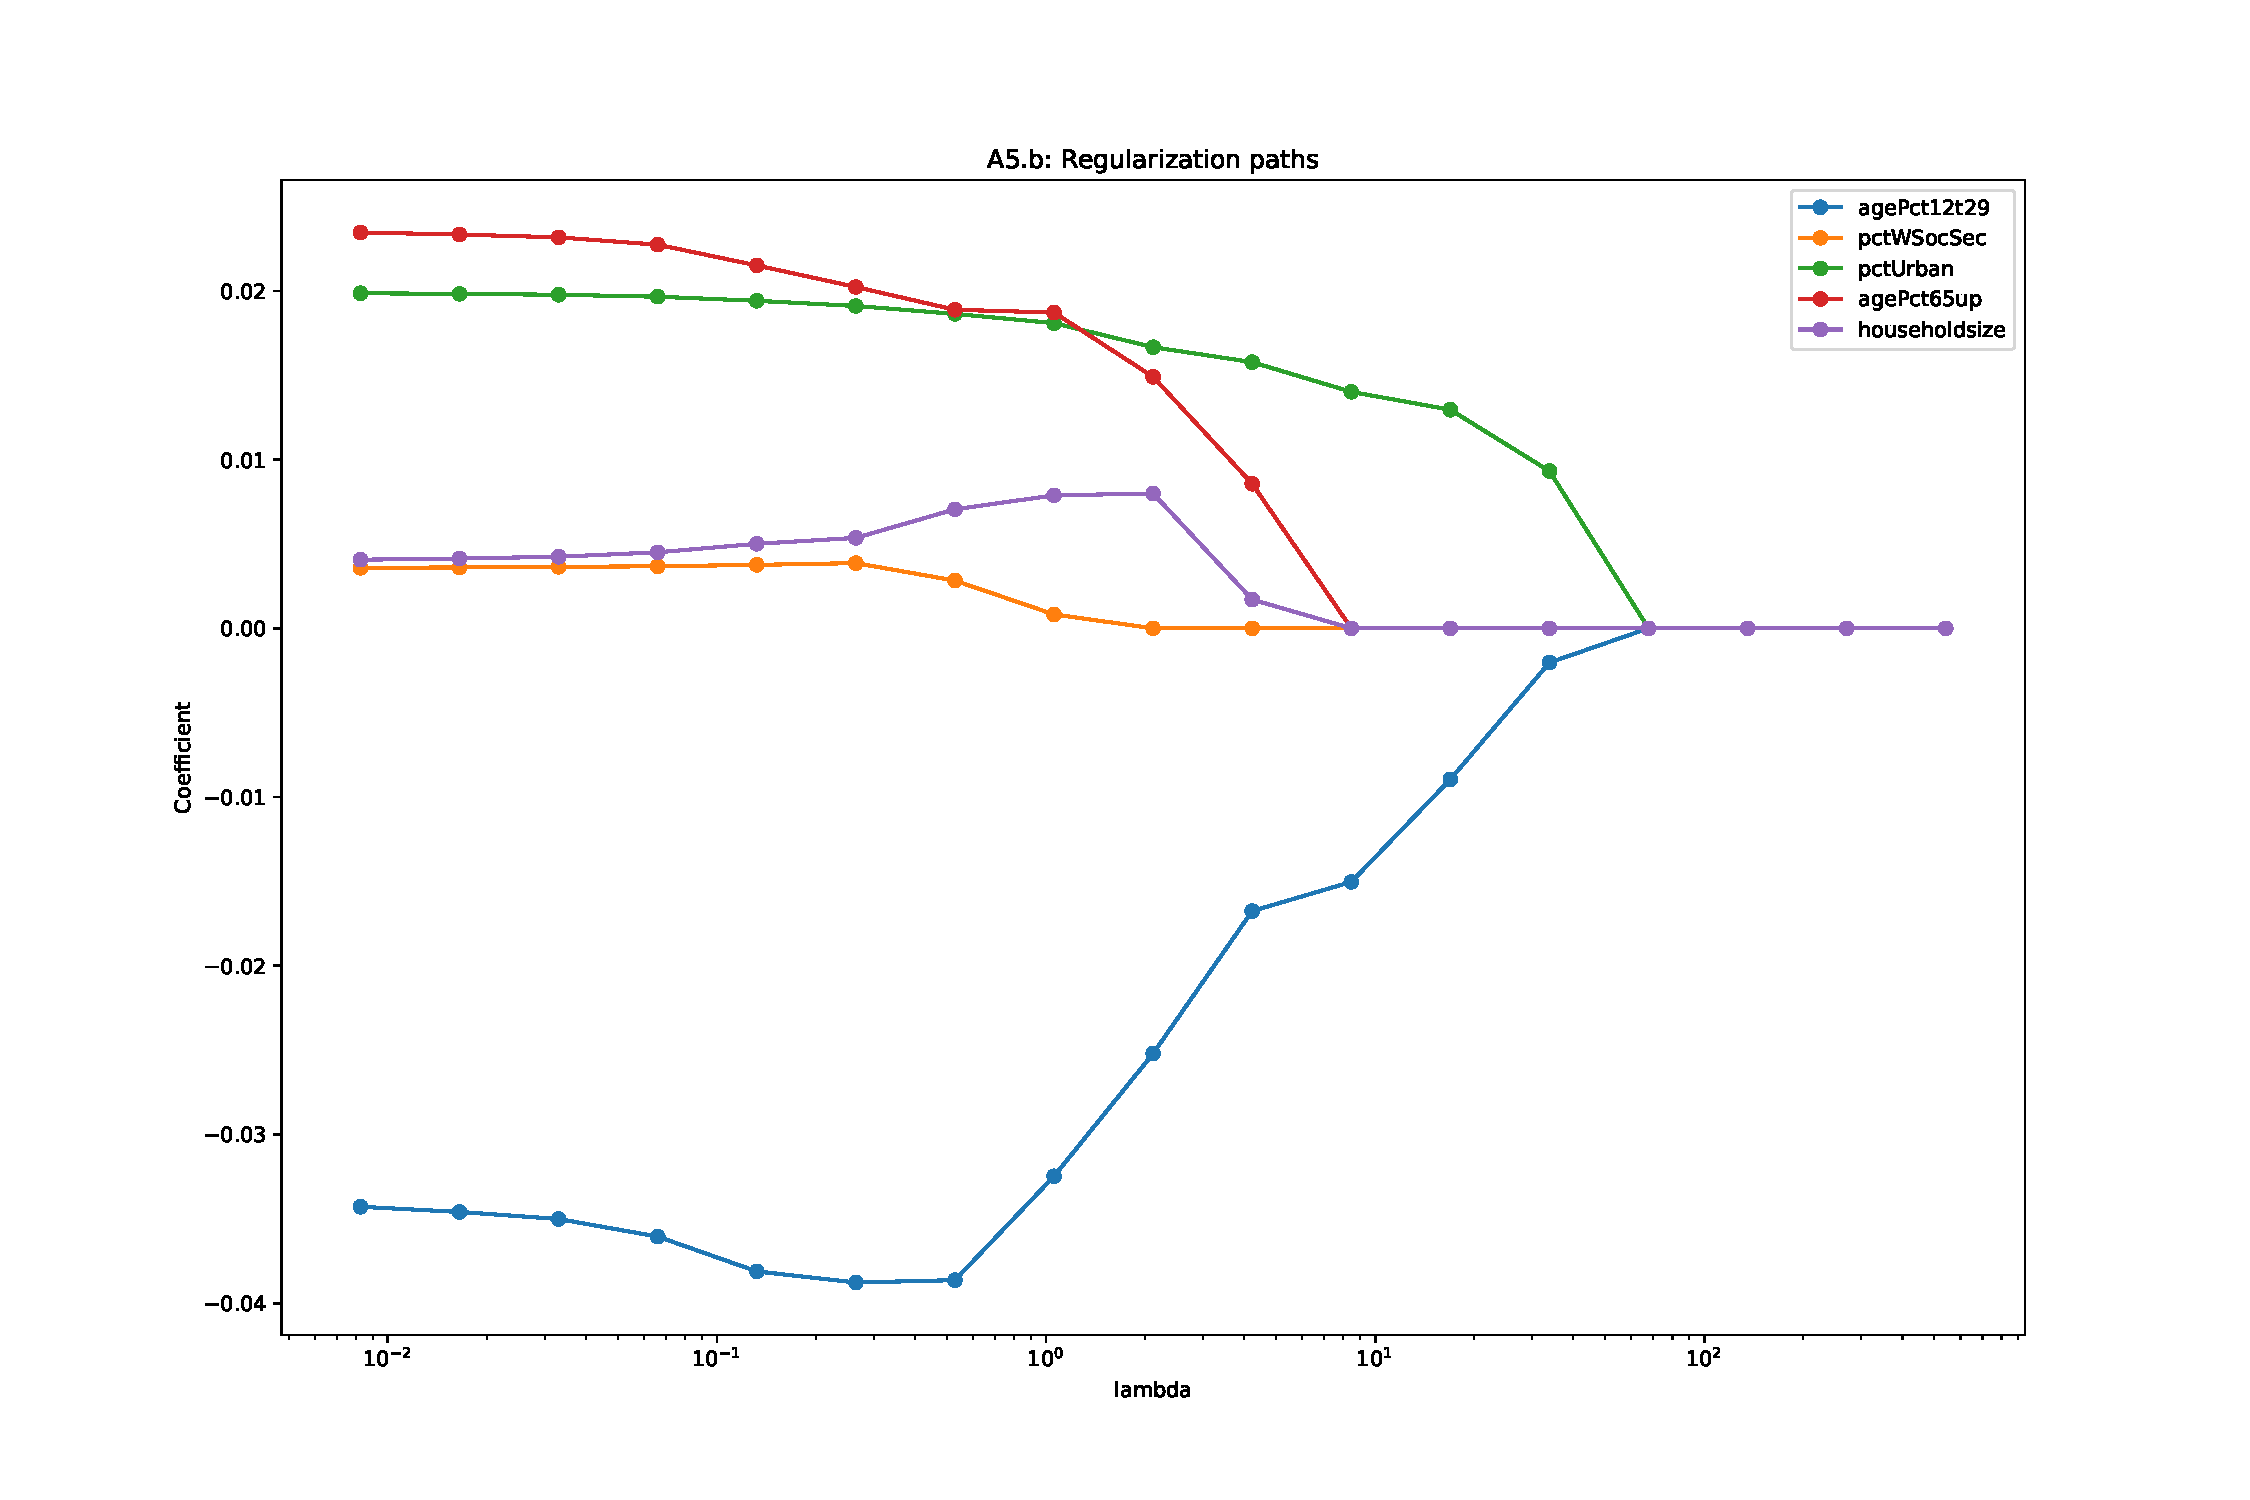
\includegraphics[width=0.49\textwidth]{hw2/code/figures/A5b.pdf}
            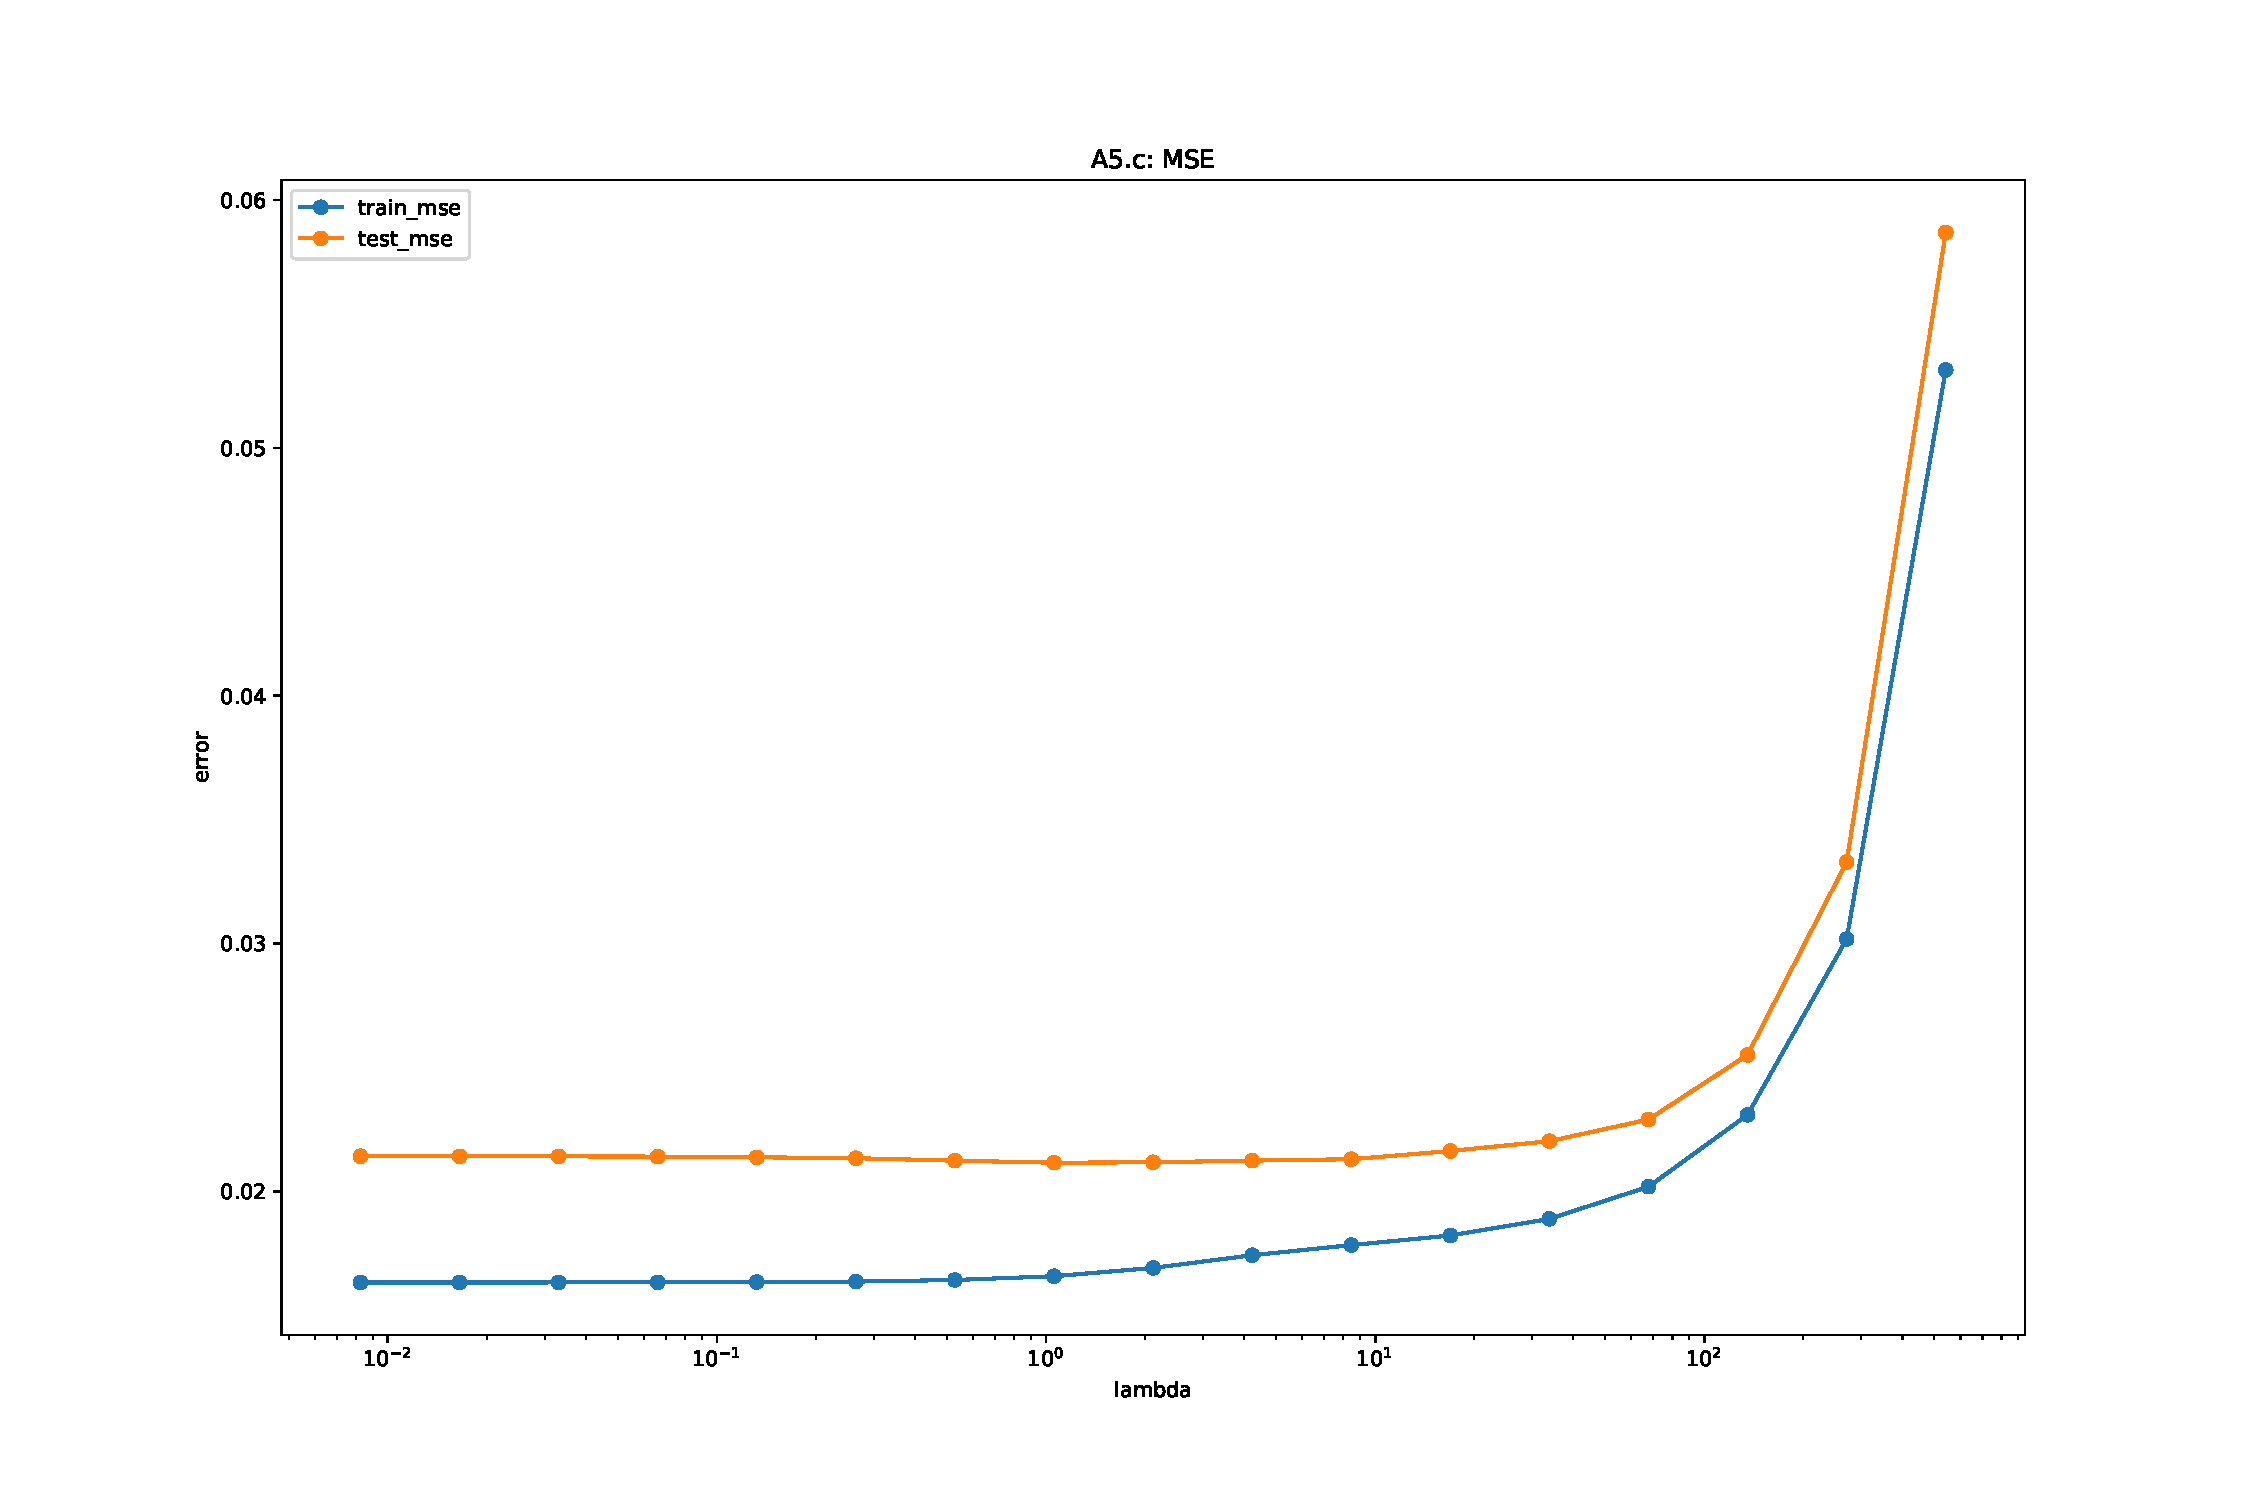
\includegraphics[width=0.5\textwidth]{hw2/code/figures/A5c.pdf}
            \caption{Problem A5. Top Left: A5.a, Top Right: A5.b, Bottom: A5.c}
            \label{figure:a4}
        \end{figure}
    \item The most positive weight: {\bf PctIlleg}\\
          The most negative weight: {\bf PctKids2Par}\\
          That is, the crime rate has the most positive correlation with PctIlleg (percentage of kids born to never married). On the other hand side, the crime rate has the most negative correlation with PctKids2Par (percentage of kids in family housing with two parents).
    \item Correlation is not the same with causality. Just because there are fewer people over 65 in the high crime areas, does not mean that the number of people over 65 decreases the crime rate. It could also mean that people over 65 tend to move out from high crime areas. Just like firetrucks don't cause fires. Seeing a fire truck is only correlated with seeing a burning building and it is the fire which causes the presence of a firetruck.

\end{enumerate}

\inputminted{python}{code/A5.py}
\caption{Code for A5}

\noindent\rule{\textwidth}{1pt}

\noindent\rule{\textwidth}{1pt}
A.6 {\bf Solution:}\\
\begin{enumerate}
    \item Note that $\exp(-y_i(b+x_i^Tw)) = \frac{1}{\mu_i(w,b)} -1$. Then, $\nabla_w J(w,b) = \frac{1}{n}\sum_i \nabla_w \log(1+\exp(-y_i(b+x_i^Tw))) + \nabla_w \lambda \|w\|^2 = \frac{1}{n}\sum_i \mu_i(w, b)(\frac{1}{\mu_i(w,b)} -1)(-y_i)x_i + 2\lambda w$. So
    $$
    \boxed{\nabla_w J(w,b) = \frac{1}{n}\sum_i (\mu_i(w, b) - 1)(y_i)x_i + 2\lambda w}
    $$
    Now, $\nabla_b J(w,b) = \frac{1}{n}\sum_i \nabla_b \log(1+\exp(-y_i(b+x_i^Tw))) + \nabla_b \lambda \|w\|^2 = \frac{1}{n}\sum_i \mu_i(w, b)(\frac{1}{\mu_i(w,b)} -1)(-y_i)$. So
    $$
    \boxed{\nabla_b J(w,b) = \frac{1}{n}\sum_i (\mu_i(w, b) - 1)y_i}
    $$
    \item See Figure 4. 
        \begin{figure}[h!]
            \centering
            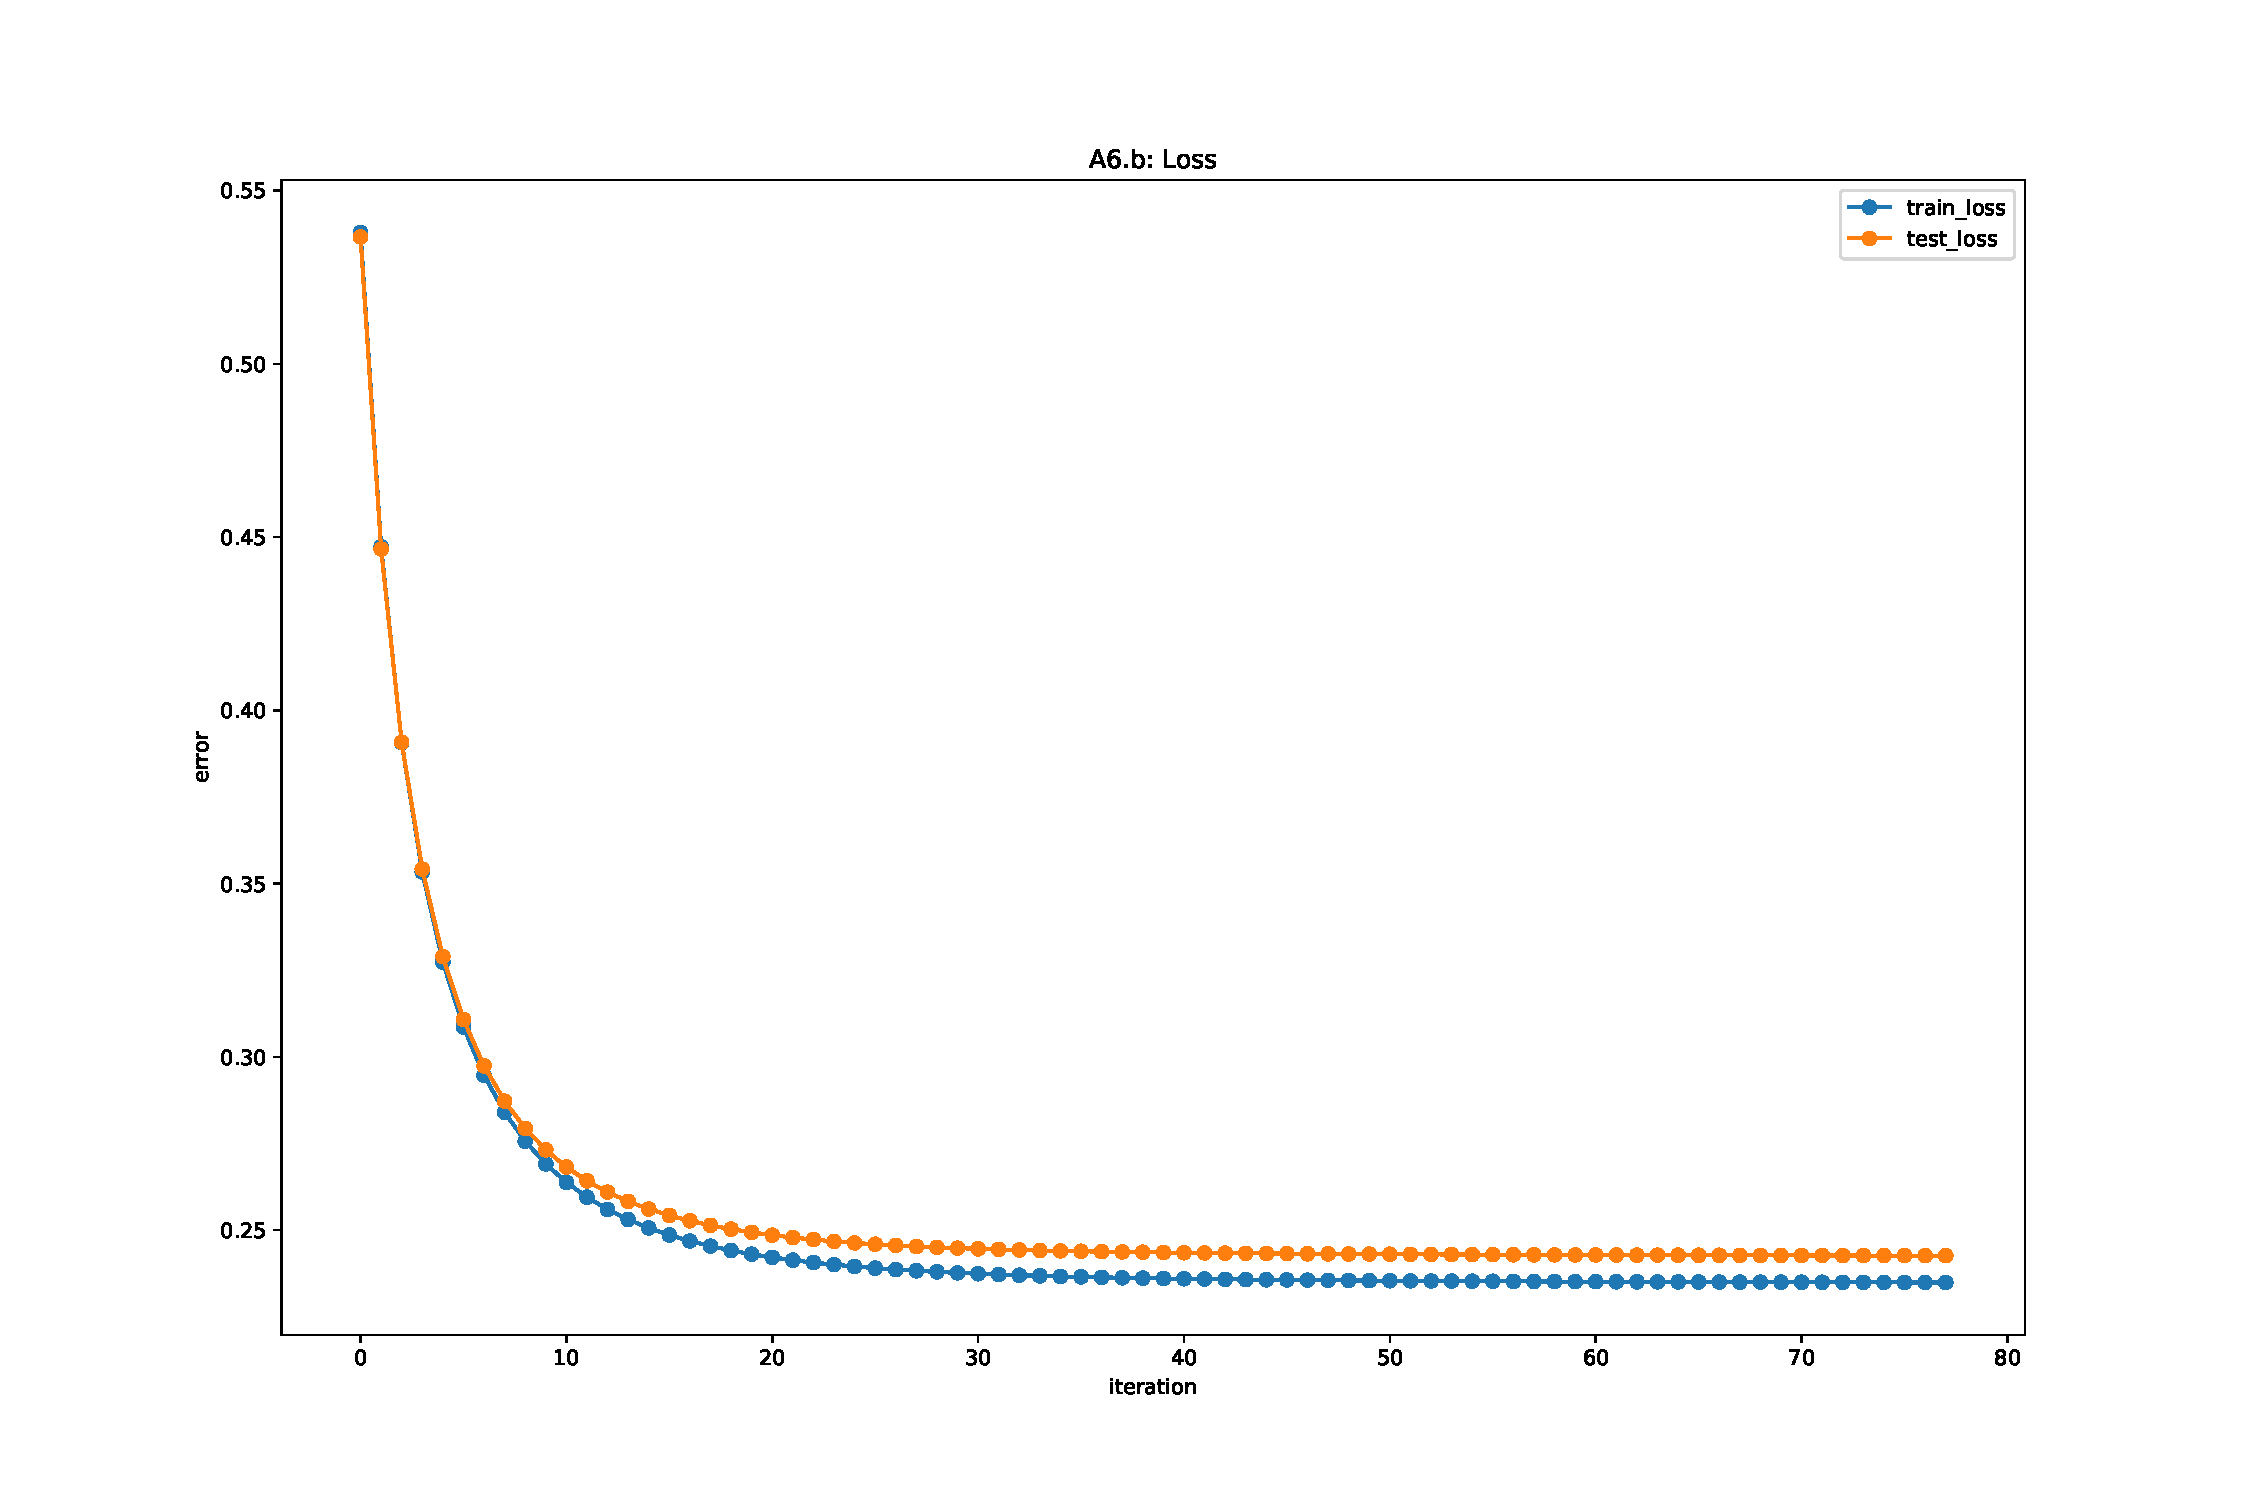
\includegraphics[width=0.49\textwidth]{hw2/code/figures/A6b1.pdf}
            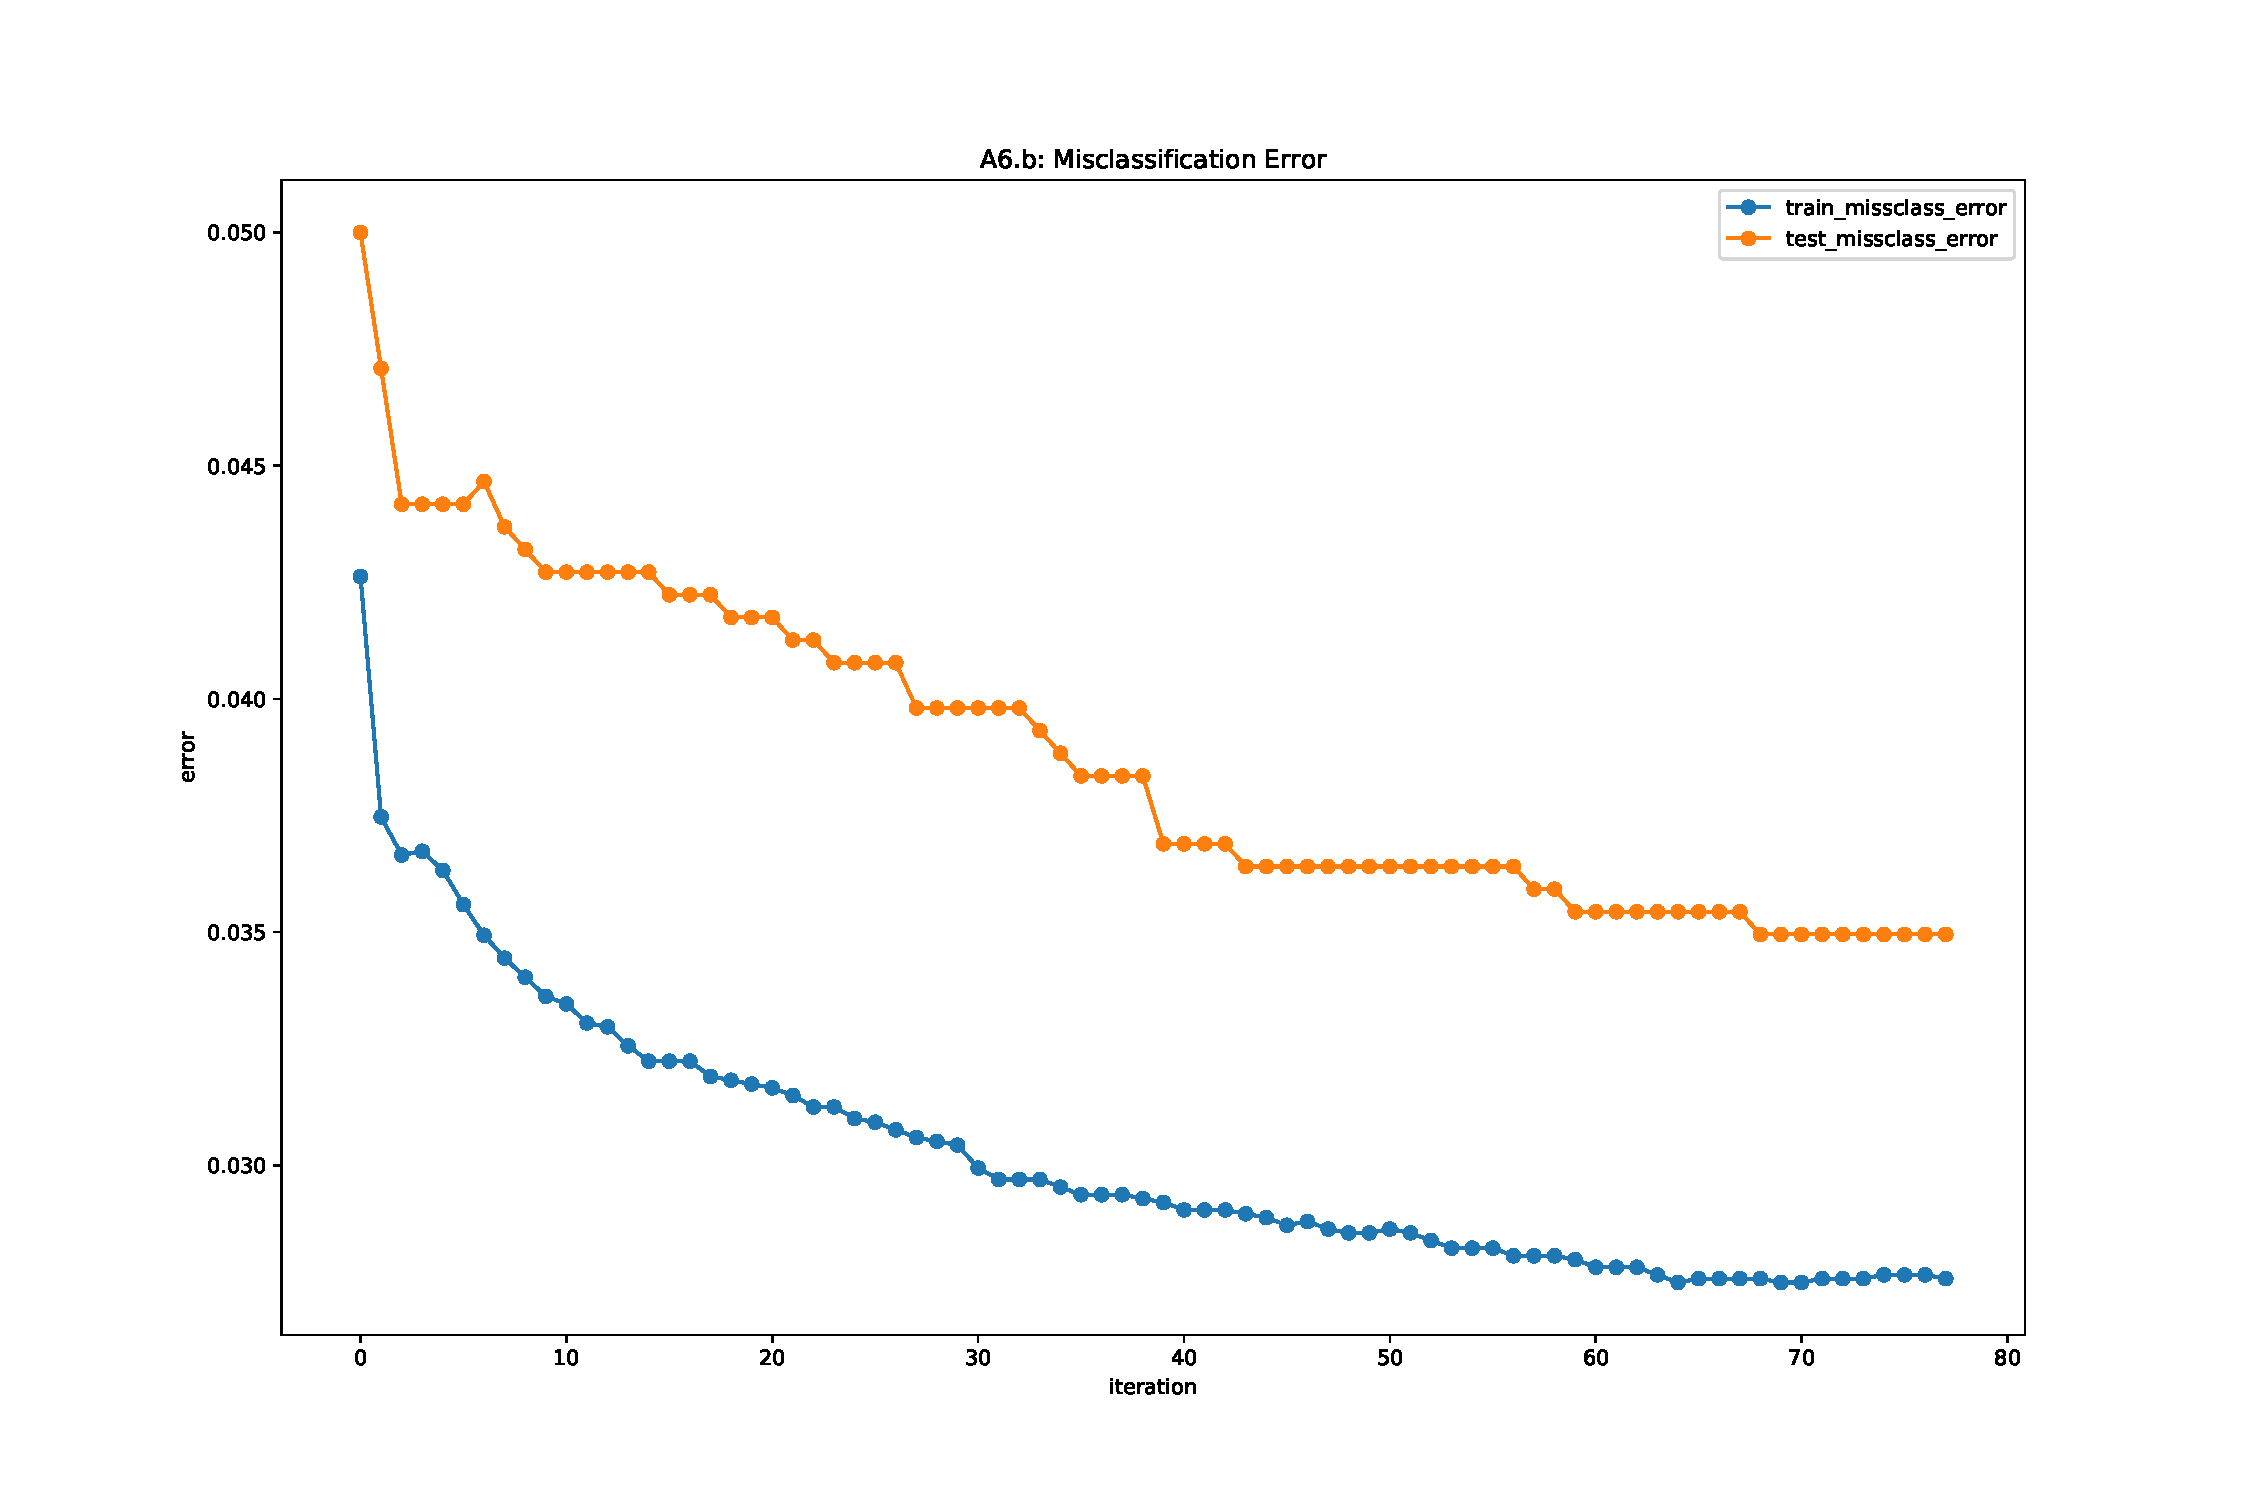
\includegraphics[width=0.49\textwidth]{hw2/code/figures/A6b2.pdf}
            \caption{Problem A6.b Left: A6.bi, Right: A6.bii (Plots for Gradient Descent)}
        \end{figure}
    \item See Figure 5. 
        \begin{figure}[h!]
            \centering
            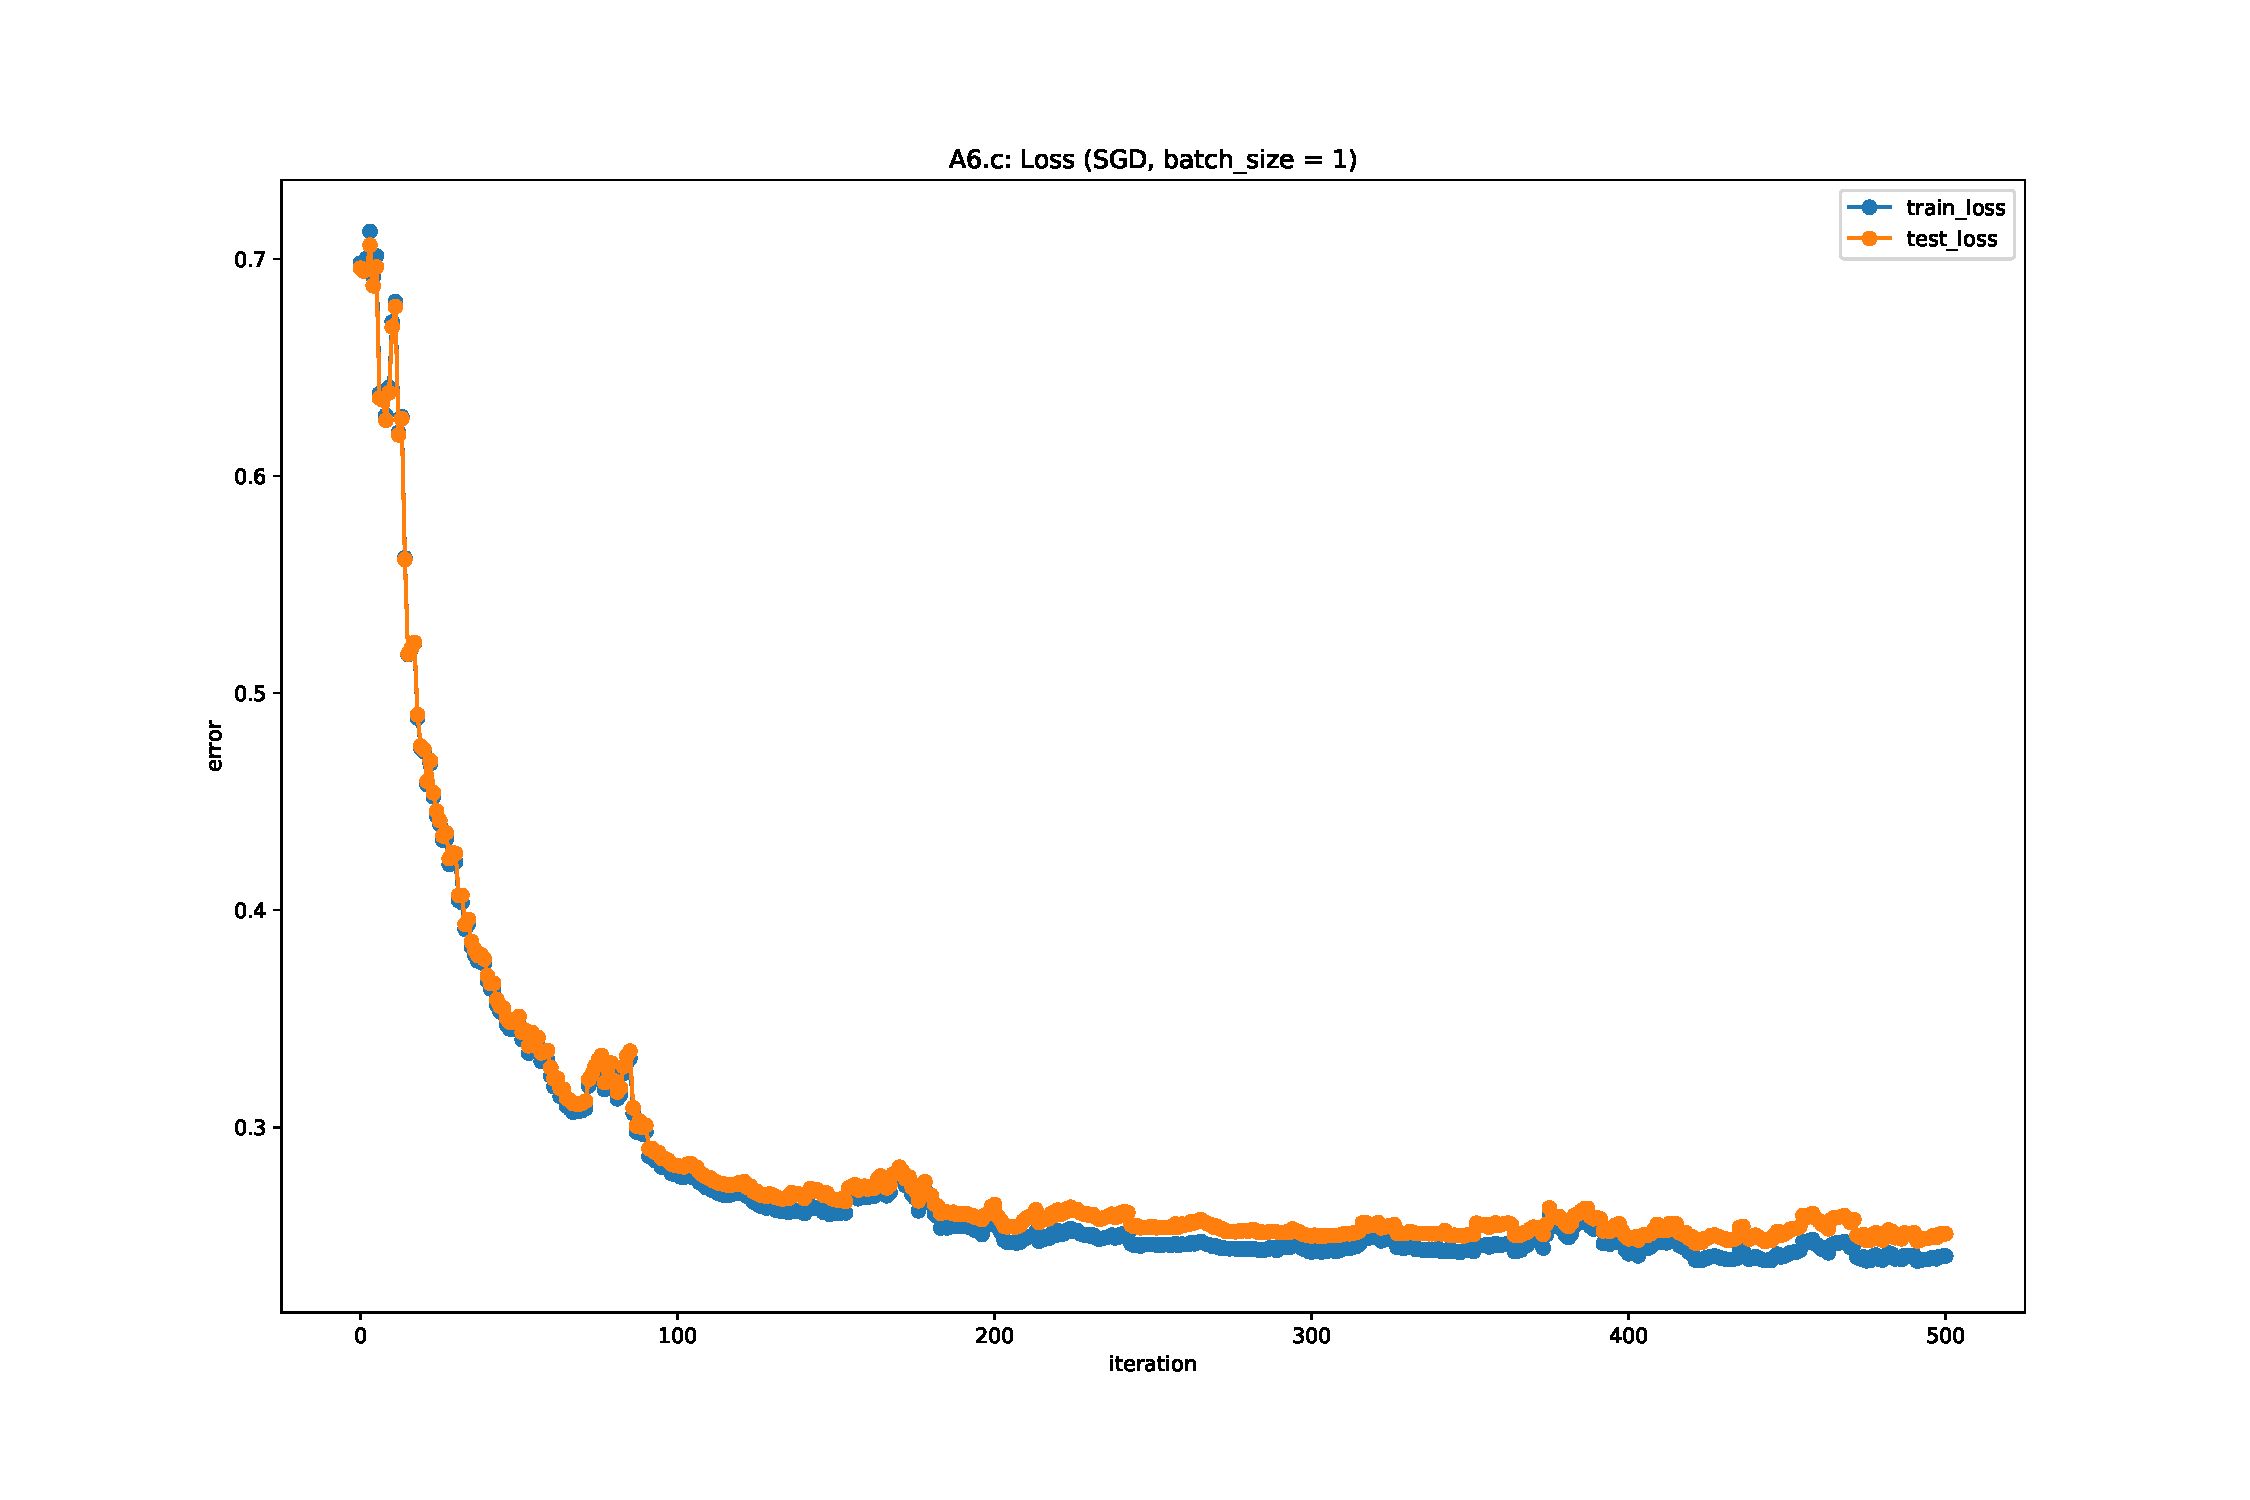
\includegraphics[width=0.49\textwidth]{hw2/code/figures/A6c1.pdf}
            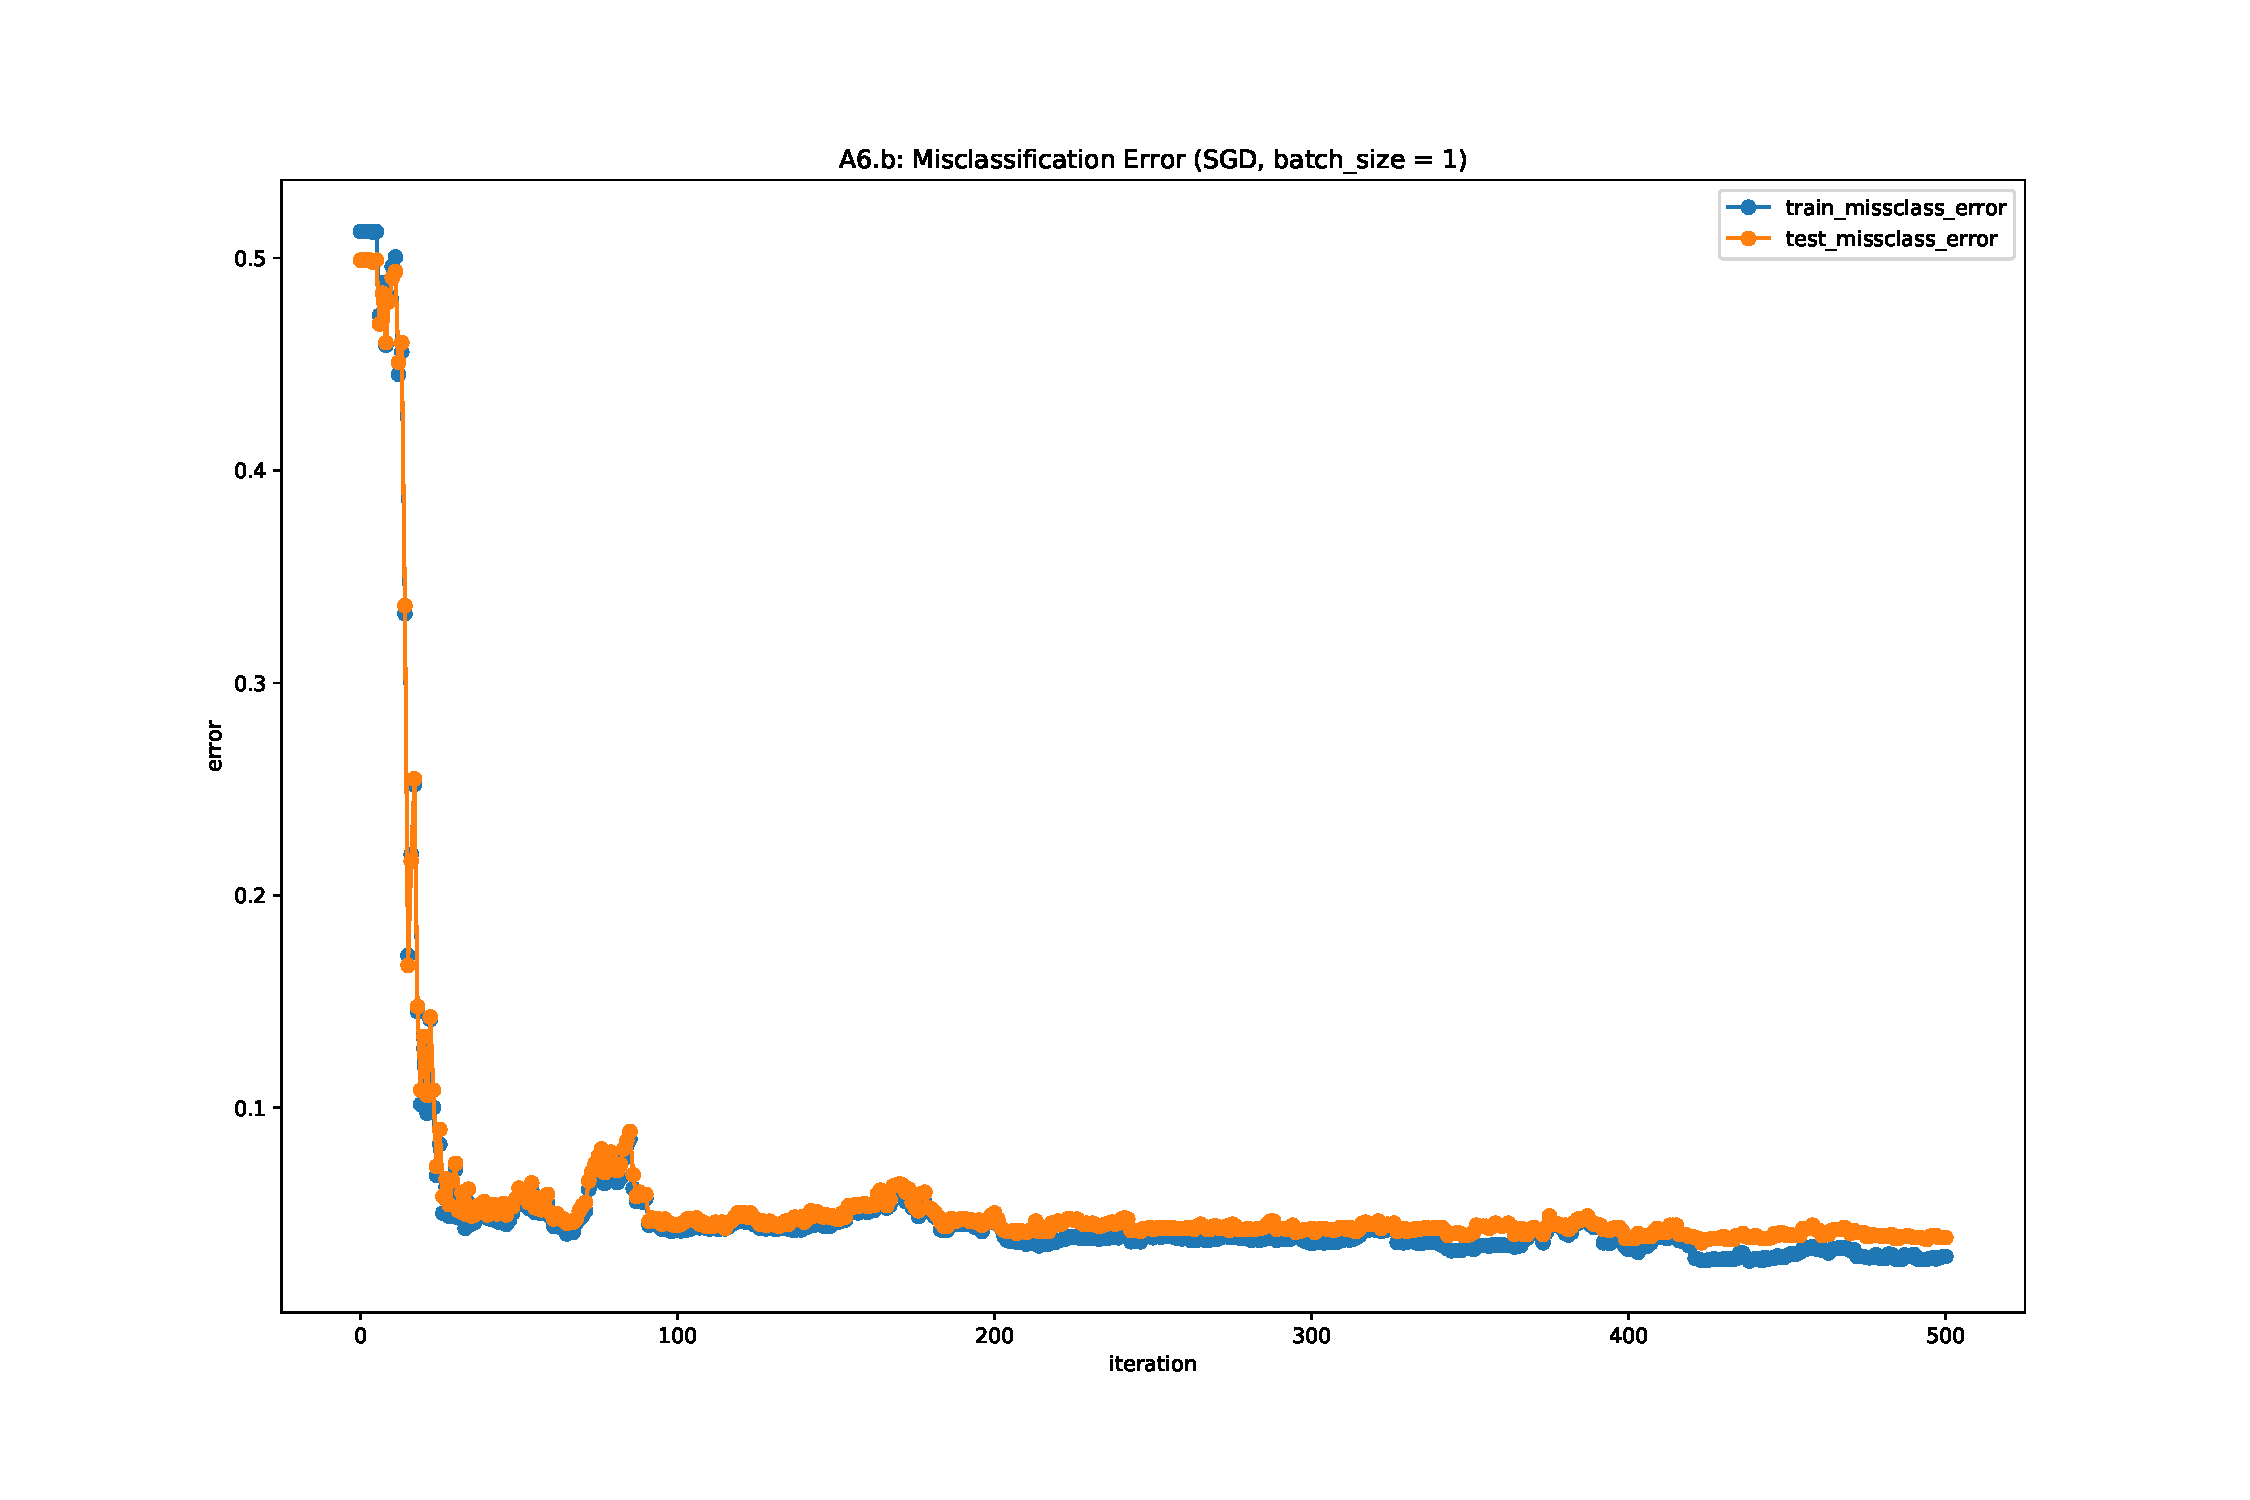
\includegraphics[width=0.49\textwidth]{hw2/code/figures/A6c2.pdf}
            \caption{Problem A6.c Left: A6.ci, Right: A6.cii (Plots for Stochastic Gradient Descent with batch 1.)}
        \end{figure}
        
    \item See Figure 6.
        \begin{figure}[h!]
            \centering
            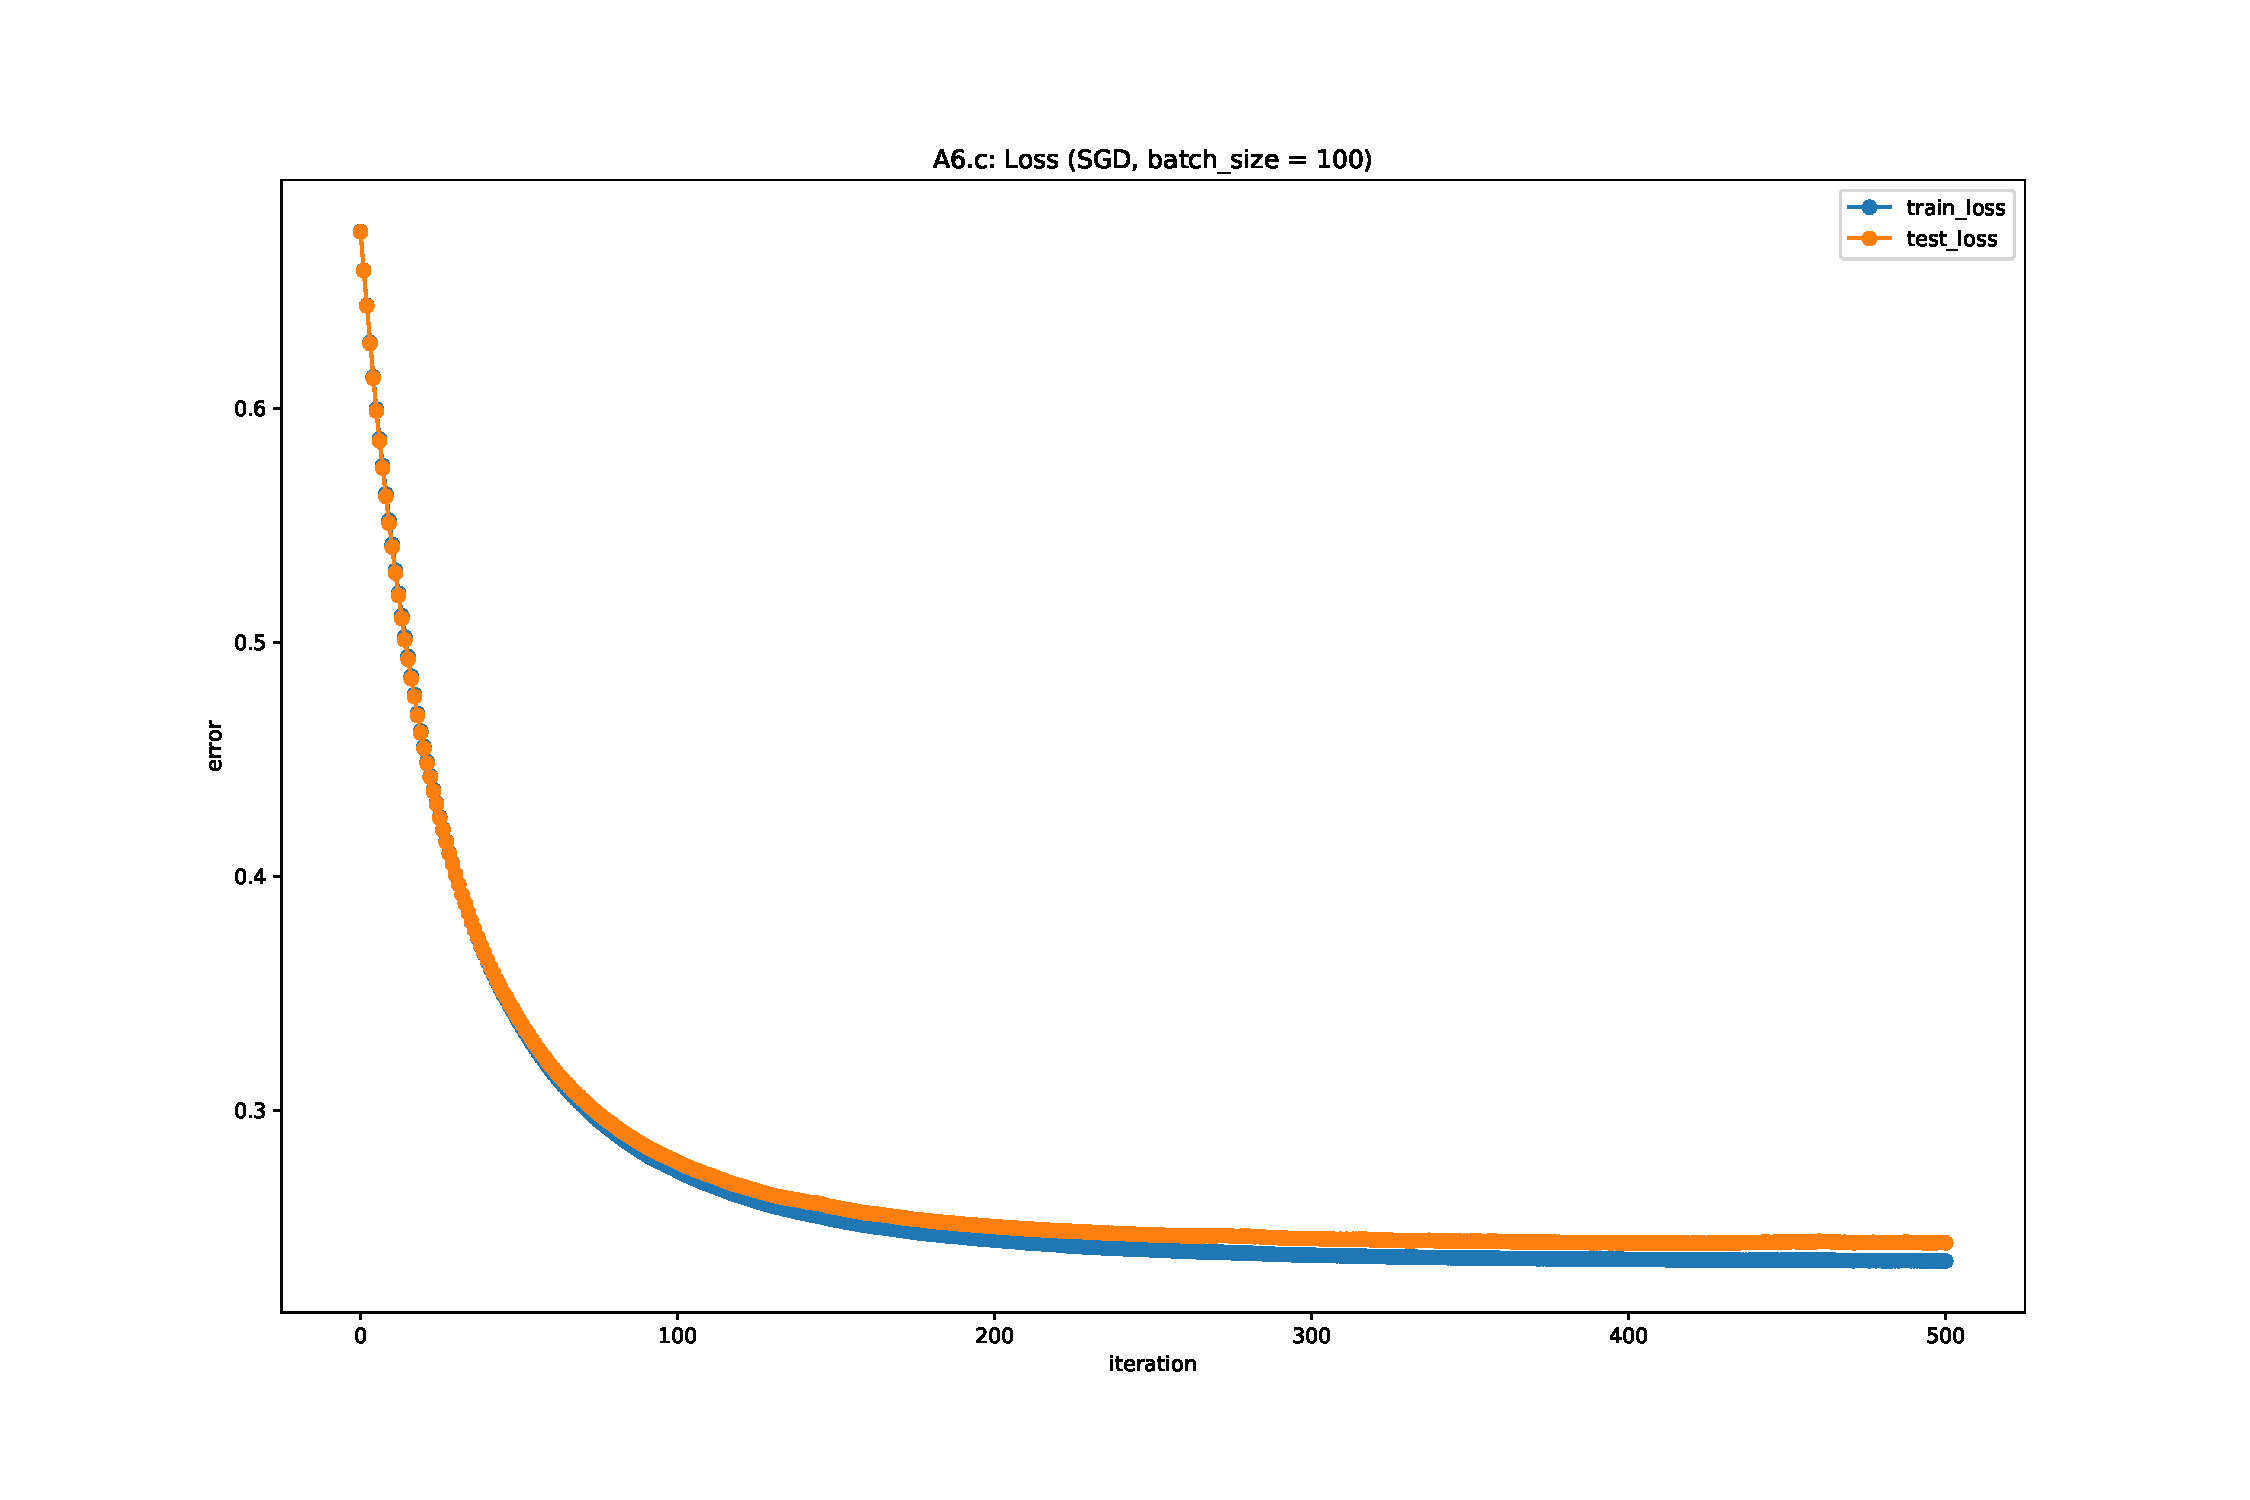
\includegraphics[width=0.49\textwidth]{hw2/code/figures/A6d1.pdf}
            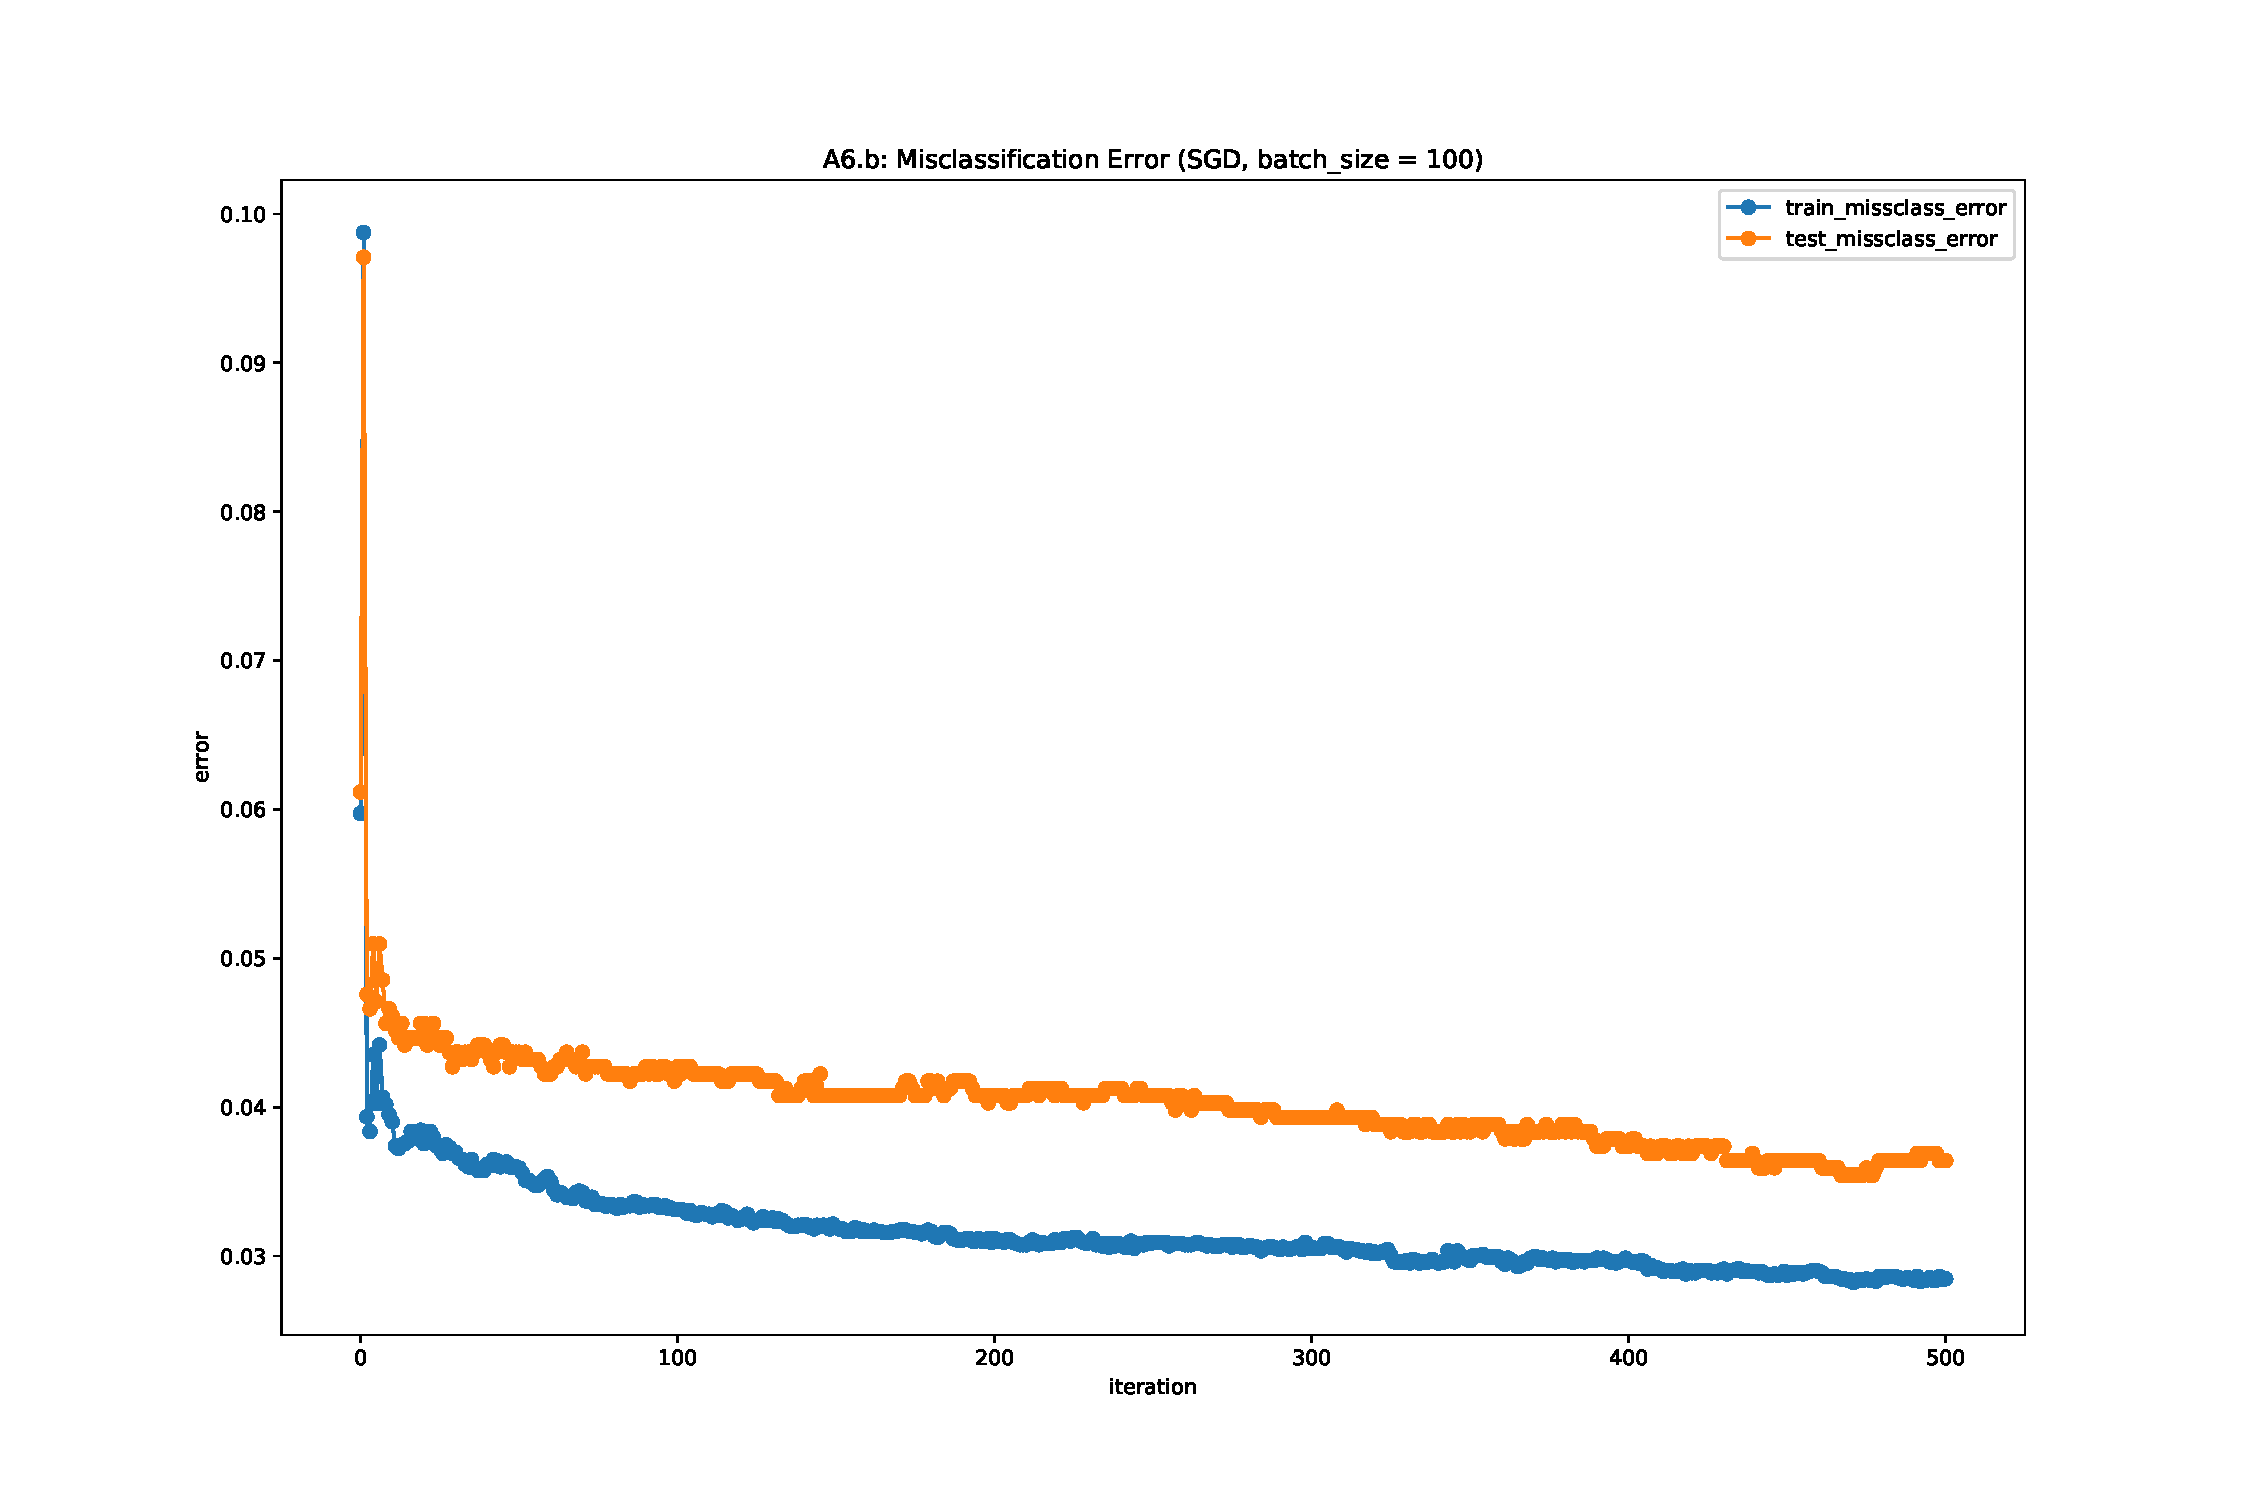
\includegraphics[width=0.49\textwidth]{hw2/code/figures/A6d2.pdf}
            \caption{Problem A6.d Left: A6.di, Right: A6.dii (Plots for Stochastic Gradient Descent with batch 100.)}
        \end{figure}

\end{enumerate}

\inputminted{python}{code/A6.py}
\caption{Code for A6}

\noindent\rule{\textwidth}{1pt}






\noindent\rule{\textwidth}{1pt}
B.4 {\bf Solution:}\\
\begin{enumerate}
    \item No time to explain!:)
    
    
    \item No time to explain!:)
    
    
    \item For Multinomial Logistic Regression trained with L(W) the train accuracy is 0.9127 and test accuracy is 0.9158. For J(W) these values are 0.8490 and 0.8537 respectively. Both models were trained for 50 epochs with learning rate $l = 0.01$. 
\end{enumerate}




\inputminted{python}{code/B4.py}
\caption{Code for B4}

\noindent\rule{\textwidth}{1pt}









\end{document}
